\documentclass[a4paper]{article}

\usepackage[english]{babel}
\usepackage[utf8]{inputenc}
\usepackage{amsmath}
\usepackage{graphicx}
\usepackage[colorinlistoftodos]{todonotes}
\usepackage{cite}
\usepackage{url}
\newtheorem{theorem}{Theorem}


\title{Summary of David Silver's Lecture on Reinforcement Learning }

\author{Jérémy Scheurer}

\date{\today}

\begin{document}
\maketitle

\begin{abstract}
This is a summary on the Lectures of David Silver on Reinforcement Learning 
\end{abstract}

\section{Introduction to Reinforcement Learning}
\begin{itemize}
\item Many branches of science have a crossover with Reinforcement Learning. This is because RL tries to solve the problem of decision making, which reappears in a lot of different sciences such as Computer science, Neuroscience, Psychology, Economy, Engineeringe etc. 
\item The difference between reinforcement learning and supervised or unsupervised learning is, that there is no supervisor which tells us what is the correct action. We only get a reward signal, and even that feedback may come much later. Time matters in RL, the learning is sequential, so we do not have i.i.d data. So what happens at one timestep correlates a lot to what happens in the next timestep. Also the agent can influence the environment and thus what it sees and learns. 
\item A reward $R_t$ is a scalar feedback signal which indicates how well an agent is doing at step t. We cannot have a vector as a reward, because in the end we should be able to lay out every action based on one reward over timesteps. The agent's job is to maximize the cumulative reward. Reinforcement learning is based on the reward hypothesis:
\begin{theorem} All goals can be described by the maximization of expected cumulative reward.
\end{theorem}
\item The goal is to select actions to maximize total future reward. It's important that one needs to plan(one cannot be greedy), because actions might have long term consequences. One might have to sacrifice immediate reward to gain more reward in the long term. 
\item We have an agent which observes observations $O_t$, it takes actions $A_t$ and receives a reward $R_t$. On the other hand we have an environment which provides the observations and reward based on the action it gets. 
\item The history is what the reward has seen so far, i.e. all the observable variables up to time t. 
$$ H_t = A_1, O_1, R_1,...A_t, O_t, R_t$$
The agent selects actions based on this history. So this history determines what it is going to happen next. But we do not want to go back through the whole history every time to predict the next action, thus we save everything in a state. 
$$ s_t = f(H_t)$$
\item The environment state $S_t^e$ is the environment's private representation. That means it is whatever data the environment uses to pick the next observation and reward. So it's not visible to the agent. Even if $S_t^e$ is visible, it may contain irrelevant information. 
\item The agent state $S_t^a$ is the agent's internal representation. That means whatever information the agent sues to pick the next action. 
\item An iformation state(a.k.a. Markov state) contains a ll useful information from the history. So we make a Markov assumption, which means that the future is independent of the past given the rpesent. 
\begin{theorem}
$P[S_{t+1}|S_t] = P[S_{t+1}| S_1,...,S_t]$
\end{theorem}
\item Fully observable environments are environments where the agent directly observes the environment state, i.e. $O_t = S_t^a = S_t^e$.
This is a Markov decision process. 
The other case is where we have a partial observability of th environment. The agent indirectly observes the environment, ex. A robot with camera vision isn't told its absolute location.  This is now a partially observable Markov decision process. 
Now the agent must construct its own state representation, ex:
\begin{itemize}
\item Complete History $S_t^a = H_t$
\item Beliefs of environment states $S_t^a = (P[S_t^e = s^1],...,P[S_t^e = s^n])$
\item Recurrent neural network: $S_t^a = \sigma(S_{t-1}^a W_s + O_t W_o)$ 
\end{itemize}
\item an RL agent my include one or more of the components: 
\begin{itemize}
\item Policy: Agent's behavior function, how it picks its action.
\item Value Function: How good is each state and/or action.
\item Model: Agent's representation of the environment.
\end{itemize}
\item A policy is the agent's behavior. it is a map from state to action, i.e. deterministic policy $a = \pi(s)$ or stochastic policy $ \pi(a|s) = P[A=a|S=s]$
\item The value function is a prediction of expected future reward. So it is used to evaluate the goodness/badness of states and therefore to select between actions. The value function is dependent on you behavior(so the policy) $$ v_{\pi}(s) = E_{\pi}[R_t + \gamma R_{t+1} + \gamma^2R_{t+2}+...|S_t = s]$$
where gamma are the discounting factors. 
\item A model predicts what the environment will do next. So its not exactly the environment, but what the agent thinks, the environment might do in the future. We could try to learn transitions which predict the next state. Or we could learn a reward model which predicts the next immediate reward. 
$$\rho_{ss}^a = P[S'=s'|S=s,A=a]$$
$$R_s^a = E[R|S=s,A=a]$$
\item We can now taxonomize RL based on these criterion's. 
\begin{itemize}
\item It's a Value Based Algorithm if it contains a value function. It could potentially only have a value function without a policy and then read out the best states. 
\item It's policy based if it only has a Policy and updates those according to the reward. 
\item Actor critic RL agent has policies and value functions. 
\item Now it can also be a model-free or model-based RL agent. 
\end{itemize}
\item There are several problems in reinforcement learning, are two of the biggest problem settings: 
\begin{itemize}
\item Reinforcement Learning Problem: The environment is initially unknown.The agent interacts with the environment and improves its policy.(Atari game)
\item Planning: A model of the environment is known. The agent performs computations with its model(without any external interaction), so it only kind of thinks. The agent then improves its policy. So this allows us to build a search tree and look ahead without actually acting.(If we had access to an emulator of the Atari game)
\item The exploration and exploitation Trade off. Reinforcement Learning is like trial and error learning. The agent should discover a good policy but it should not give up opportunity of exploiting what is has discovered.
\item The final problem is prediction and control. Prediction means to evaluate the future with a given policy. Control means to optimize the future i.e. find the best policy. In RL usually we have to solve the prediction problem to solve the Control problem. 
\end{itemize}
\end{itemize}

\section{Markov Decision Processes}
\begin{itemize}
    \item Markov decision process formally describes an environment for reinforcement learning where the environment is fully observable, i.e. the current state completely characterizes the process. Almost all RL problems can be formalized as MDP's. Even partially observable problems can be converted into MDP's. 
    \item The central property of an MDP is the Markov property(see Markov Theorem). For a Markov state s and successor state s', the state transition probability is defined by $$P_{ss} = P[S_{t+1} = s' | S_t = s]$$
    \begin{theorem}
    A Markov process is a memoryless random process, i.e. a sequence of random states S1, S2, ... with the Markov property. So a Markov Process is a Tuple $<S,P>$, where S are a set of finite states and  is a state transition probability matrix. 
    \end{theorem}
    \item 
    \begin{theorem}
        A Markov reward process is a Markov chain with values. It is a Tuple $< S, P, R, \gamma>$, where S is a finite set of states, P is a state transition probability matrix, R is a reward function $R_s = E[R_{t+1}|S_t = s]$ and $\gamma \epsilon [0,1]$ is a discount facto.
    \end{theorem}
    \item The goal of RL is to maximize the return $G_t$ which is the total discounted reward from time step t. $$G_t = R_{t+1} + \gamma R_{t+2} + ... = \sum_{k=0}^{\infty} \gamma^k R_{t+k+1}$$
    \item Why should we use a discount factor? Because we cannot trust our decisions fully, because we only have a model of the environment and we cannot be perfectly certain about the future. Also its mathematically convenient and avoids infinite returns in cyclic Markov processes. Also if the reward is financial, immediate rewards may earn more interest than delayed rewards. Cognitively animals and humans prefer immediate rewards. 
    If all possible return sequences are finite we can omit discounting. 
    \item 
    \begin{theorem}
    Value function v(s) gives the long term value of state s. So the state value funciton of an MRP is th eexpected return starting from state s: $$ v(s) = E[G_t|S_t = s]$$
    \end{theorem}
    \item 
    \begin{theorem}
    The Bellman Equation for MRP's. The value funciton can be decomposed into two parts: immediate reward $R_{t+1}$ and discounted value of successor state: 
    $$v(s) = E[G_t | S_t = s]$$
    $$= E[R_{t+1} + \gamma R_{t+2} + y^2 R_{t+3}+ ... | S_t = s]$$
    $$= E[R_{t+1} + \gamma R_{t+2} + y^2 R_{t+3}+ ... | S_t = s]$$
    $$= E[R_{t+1} + \gamma(R_{t+2} + y R_{t+3}+ ...) | S_t = s]$$
    $$= E[R_{t+1} + \gamma G_{t+1}| S_t = s]$$
    $$= E[R_{t+1} + \gamma v(S_{t+1}) | S_t = s]$$
    \end{theorem}
    In other words: $$ v(s) = R_s + \gamma \sum_{s'\epsilon S} P_{ss'}v(s')$$
    \item The Bellman equation can be formulated in a vector/matrix formulation: $v = R + \gamma v$ where $v \epsilon R^n, R \epsilon R^n, P \epsilon R^{n,n}$
    The Bellman equation is a linear equation and can directly be solved. This is not going to be true for Markov Decision Processes. It only works for evaluating rewards, if we want to maximize rewards, its not possible anymore. 
    $$v = (I-\gamma P)^{-1} R$$
    Note that the computational complexity is $O(n^3)$ for n states. Direct solutions only possible for small Markov reward Processes. There are many iterative methods for lagre MRP's such as Dynamic programming, Monte-Carlo evaluation and Temporal-Difference learning. 
    \item Now we look at what we actually use in RL which are Markov decision Processes. 
    \begin{theorem}
    A Markov decision process is a Markov reward process with decisions. It is an environment in which all states are Markov. It is a tuple $<S, A, P, R, \gamma>$ where S is a finite set of states, A is a finite set of actions, P is a state transition probability matrix, $\gamma$ is a discount factor, R is a reward function, $R_s^a = E[R_{t+1} | S_t = s, A_t = a]$ and $P_{ss'}^a = P[S_{t+1} = s' | S_t = s, A_t = a]$.
    \end{theorem}
    \item So now we want to find a path(select actions) through our MDP which maximizes the rewards. To do this we need a Policy which fully defines the behaviour of an agent. 
    \begin{theorem}
    A policy $\pi$ is a distribution over actions given states:
    $$\pi(a|s) = P[A_t = a|S_t=s]$$
    \end{theorem}
    \item Policies are stationary, i.e. time-independent. 
    \item Note the connection between an MDP and a MRP is the following. If we fix a policy and sample a state sequence, this sequence is a Markov process. The state and reward sequence we get is a Markov reward Process. In other words one takes the average of the dynamics as an MRP, i.e. 
    $$ P_{s,s'}^{\pi} = \sum_{a\epsilon A} \pi(a|s)P_{s,s'}^a$$
    $$R^{\pi}= \sum_{a\epsilon A} \pi(a|s)R_{s}^a$$
    \item How good is it to be in a certain state. 
    \begin{theorem}
    The state-value function $v_{\pi}$ of an MDP is the expected return starting from state s, and then following policy $\pi$ $$ v_{\pi}(s) = E_{\pi}[G_t |S_t=s]$$
    \end{theorem}
    \item How good is it to take a specific action in a certain state. 
    \begin{theorem}
    The action value function $q_{\pi}(s,a)$ is the expected return starting from state s, taking action a, and then following policy $\pi$ 
    $$q_{\pi}(s,a)= E_{\pi}[G_t | S_t = s, A_t = a]$$
    \end{theorem} 
    \item The state-value function can again be decomposed into immediate reward plus discounted value of successor state. 
    \begin{theorem}
    Bellmann-Equation: $$v_{\pi}(s) = E_{\pi}[R_{t+1} + \gamma v_{\pi}(S_{t+1}) | S_t = s]$$
    The action value function can similarly be decomposed: 
    $$q_{\pi}(s,a) = E_{\pi}[R_{t+1} + \gamma q_{\pi}(S_{t+1}, A_{t+1}) | S_t = s, A_t = a]$$ 
    \end{theorem}
    \item How do V and Q relate to each other? 
    $$v_{\pi}(s) = \sum_{a\epsilon A}\pi(a|s)q_{\pi}(s,a)$$ 
    $$q_{\pi}(s,a) = R_s^a + \gamma\sum_{s'\epsilon S}P_{ss}^a v_{\pi}(s')$$
    You can now insert the second equation into the first equation which gives the Bellmann equation. You could also insert the first equation into the second equation. The difference is in the first method you go from a state and you say okay what different actions could I take. And then you ask after taking these actions where might the wind blow you. For the second method you consider a specific action and wonder where the wind might blow you and from that state you consider all possible actions you could take. 
    \item But what we now want is not to have any policy but the best policy. 
    \begin{theorem}
    The optimal state-value function $v_{*}$ is the maximum value funciton over all policies: 
    $$ v_{*}(s) = max_{\pi}v_{\pi}(s)$$
    The optimal action-value function $$q_{*}(s,a) = max_{\pi} q_{\pi}(s,a)$$ 
    The optimal value function specifies the best possible performance in the MDP. And MDP is "solved" when we know the optimal value function. 
    \newline
    If you think of it, you are trying to find the policy which maximizes the rewards you get in this system and thus maximizes the expected return starting from state s and following policy $\pi$(state value function). Or in other words, under every possible policy, we will get a specific state value function which is maximal. 
    \newline
    Also if you have the optimal action-value function you are basically done, because you can insert any action possible and then choose the one with the larges action value function. 
     \end{theorem}
    \item We are interested in the optimal policy which is just a function from states to actions. So to find a best we need to introduce a partial ordering of policies. $\pi >= \pi'$ if $v_{\pi}(s) >= v_{\pi'}(s)$, fo rall s. 
    \begin{theorem}
    For any Markov Decision Process: 
    \begin{itemize}
        \item There exists and optimal policy $\pi_{*}$, that is better than or equal to all other policies. 
        \item All optimal policies achieve the optimal value function, $v_{\pi_{*}} = v_*(s)$
        \item All optimal policies achieve the optimal action -value function, $q_{\pi_{*}}(s,a) = q_*(s,a)$
    \end{itemize}
    \end{theorem}
    \item An optimal policy can be found by maximizing over $q_*(s,a)$, i.e. 
    $$\pi_*(a|s) = 1 if a = argmax_{a\epsilon A}q_*(s,a)$$ and 0 otherwise
    \item How can we figure out $q_*$? 
    \begin{theorem}
    The optimal value functions are recursively related by the Bellman optimality equations: 
    $$v_*(s) = max_a q_*(s,a)$$
    $$q_*(s,a) = R_s^a + \gamma \sum_{s'\epsilon S}P_{ss'}^a v*(s')$$
    We can now again insert the second term in the first term or the first into the second. 
    \end{theorem}
    \item Bellman Optimality Equation is non-linear, how can we solve it? There are many iterative solution methods such as value iteration, policy iteration, Q-learning and Sarsa. 
\end{itemize} 

\section{Planning by Dynamic Programming}
\begin{itemize}
    \item There are different ways of planning, here a few of them we will look at. Policy evaluation, which means given a certain policy, how good is this policy. Then there is policy iteration which takes the idea of policy evaluation to find the best policy. Value iteration optimizes the Bellmann Equation.  
    \item What is dynamic programming? It is optimizing a mathematical policy which has a sequential or temporal component to the problem. You can divide your problem into substructures and solve these. A DP needs two properties. First of all the principle of optimality, i.e. solving the sub-problems also solves the initial problem. The second is overlapping sub-problems which means that one sub-problem is a sub-problem for different initial problems. 
    \newline
    Luckily a MDP satisfies both properties. The Bellman equation gives recursive decomposition. The value functions stores and reuses solutions. 
    \item The difference between RL and Planning is that in planning, we know the transition and reward structures and try to find the optimal policy.
    \item DP assumes full knowledge of the MDP and is used for planning.
    \begin{itemize}
        \item For prediction we have the input $(<S,A,P,R,\gamma)$ and a policy $\pi$, the output is $v_{\pi}$. So this is something like policy evaluation.
        \item For control(what we really want to find out): 
        The input is  $(<S,A,P,R,\gamma)$ and the output is the optimal value function $v_*$ and $\pi_*$, so the most reward we can get and thus also what is the best policy. 
    \end{itemize}
\end{itemize}
\subsection{Policy Evaluation}
\begin{itemize}
    \item Here we use the Bellman expectation equation and for the Control problem we use the Bellman optimality equation. The problem we have here is to evaluate a given policy $\pi$. So we will start with an initial value function and iterate the Bellman expectation backup. 
    \item Synchronous Backups: At each iteration $k+1$ for all states s, update $v_{k+1}(s)$ from $v_k(s')$, where s' is a successor state of s. That means we iteratively calculate the following: 
    $$v_{k+1}(s) = \sum_{a \epsilon A} \pi (a|s)(R_s^a + \gamma \sum_{s' \epsilon S} P_{ss'}^a v_k(s'))$$
    \item If we look at a grid example we can iteratively apply the expectation Bellman equation to find the true value function for the states. One can then learn new policies by acting greedely and always move around according to the best states. But note that here we improved a policy, but the state value improvement with the Bellman equation always assumed a random policy. This now leads us to the next topic. 
\end{itemize}
\subsection{Policy Iteration}
\begin{itemize}
    \item The goal is to find an optimal policy given a policy $\pi$. How can we improve the policy: 
    \newline
    Evaluate the policy $\pi$:
    $$v_{\pi}(s) = E[R_{t+1} + \gamma R_{t+2}+ ...| S_t = s]$$
    Then improve the policy by acting greedily with respect to $v_{\pi}$
    $$\pi' = greedy(v_{\pi})$$
    In our grid world example we only had to go through the algorithm once to get the optimal policy. But usually we need to do this several times to get smoothing optimal. 
    \item Why do we find the optimal policy with this algorithm? Consider a deterministic policy, $a = \pi(s)$. We can improve the policy by acting greedily: $ \pi'(s) = argmax_{a \epsilon A} q_{\pi}(s,a)$. This imprpoves the value from any state s over one step, $$q_{\pi}(s,\pi'(s)) = max_{a \epsilon A} q_{\pi}(s,a) >= q_{\pi}(s,\pi(s)) = v_{\pi}(s)$$
    With a telescoping prove one can then show that it therefore improves the value function, i.e. $ v_{\pi'}(s) >= v_{\pi}(s)$
    Proof: 
    $$v_{\pi}(s) <= q_{\pi}(s, \pi'(s)) = E_{\pi'}[R_{t+1} + \gamma v_{\pi}(S_{t+1})| S_t = s ]$$
    $$<= E_{\pi'}[R_{t+1} + \gamma q_{\pi}(S_{t+1}, \pi'(S{t+1})))| S_t = s ] $$
    $$<=E_{\pi'}[R_{t+1} + \gamma R_{t+2} + \gamma^2 q_{\pi}(S_{t+2}, \pi'(S_{t+2}))| S_t = s]$$
    $$E_{\pi'}[R_{t+1} + \gamma R_{t+2} + ... |S_t =s] = v_{\pi'}(s)$$
    \newline
    At some point this iterative method is going to stop because it is equally good as the last step. How can we now prove, that this is the optimal policy? 
    If improvements stop, 
    $$q_{\pi}(s, \pi'(s)) = max_{a\epsilon A} q_{\pi}(s,a) = q_{\pi}(s, \pi(s)) = v_{\pi}(s)$$
    In which case the Bellman optimality equation has been satisfied because : $$v_{\pi}(s) = max_{a \epsilon A} q_{\pi}(s,a)$$
    \item We saw in the grid world that improving the state value function only a little bit already got us the best optimal policy. So how could we use this and not calculate our algorithm till the end. We could introduce a stopping condition epsilon which looks at convergence of the value function. But even that would waste some effort. So what we could do is to evaluate a policy k-times(improve the value function) and after k steps improve the policy. This also converges to the optimal policy. 
    The extreme case of this is to update the policy every iteration, i.e. stop after k = 1. This is equivalent to value iteration.  
\end{itemize}
\subsection{Value iteration}
\begin{itemize}
    \item Any optimal policy can be subdivided into two components, an optimal first action A*, followed by an optimal policy from successor state S'. 
    \begin{theorem}
    principle of Optimality for policies: 
    A policy $\pi(a|s)$ achieves the optimal value from state s, $v_{\pi}(s) = v_*(s)$ if and only if for any state s' reachable from s, $\pi$achieves the optimal value from state s', i.e. $v_{\pi}(s') = v_*(s')$
    \end{theorem}
    \item If we know the solution to subproblems $v_*(s')$. Then solution $v_*(s)$ can be found by one-step lookahead: 
    $$v_*(s) <- max_{a \epsilon A} R_s^a + \gamma \sum_{s'\epsilon S}P_{ss'}^a v_*(s')$$
    You have to note that the idea of having a final state and working backwards is only for the intuition. The algorithm also works if there is no final state and also if we don't know the final state. 
    \newline
    The idea is that each state gets to be the root state. We then initiate all states with some value function(ex. 0). Then for all states(where each individual state is considered to be the root state) we take the max action, which maximizes a one step look ahead of what the environment could do based on this action(where the wind might bring us). 
    \item So in value iteration we try to find the optimal policy in the planning problem(not RL problem). The solution is to iteratively apply the Bellman optimality backup. Also note that before(policy iteration) we applied the Bellman expectation equation which found us the value function for a given policy. No we iterate the Bellman optimality backup which finds us the optimal value function. 
    \item So what is the difference between policy iteration and value iteration? In value iteration, we do not explicitly build a policy at each iteration. Also if you just stop at any value iteration, this value function might not be meaningful for a specific policy, but in the end it will. Also remember that this is equivalent to policy iteration with k = 1. So you evaluate the expected Bellman equation at each step for a new greedy policy which is the argmax and which then yields a max. 
    \item So to summarize what we have done until now, this were all synchronous dynamic programming algorithms. 
    \begin{itemize}
        \item Prediction: Use Bellman Expectation Equation (iterative policy evaluation). 
        \item Control: Use Bellman Expectation Equation + Greedy Policy Improvement (Policy iteration)
        \item Bellman Optimality Equation (Value Iteration). 
    \end{itemize}
    All algorithms are based on state value function $v_{\pi}(s)$ or $v_*(s)$. The complexity is $O(mn^2)$ per iteration for m actions and n states. One could also apply it to action-value functions $q_{\pi}(s,a)$ or $q_*(s,a)$ which would then have a complexity of $O(m^2n^2)$ per iteration. 
\end{itemize}
\subsection{Extensions to Dynamic Programming}
\begin{itemize}
    \item Do you have to look at every single state in your iteration(i.e. all states are backed up in parallel)? No. You can do it asynchronously. So for each selected state, apply the appropriate backup. It will also converge as long as you still select all states frequently, but the order does not matter. 
    \item In-place dynamic programming. You always have to store the old and the new value of your value function for synchronous value iteration. In-place value iteration just uses one memory location for the new and old value functions. That is you just replace the old one by the new one. But you still have a value function for each state. 
    \item Prioritized sweeping tries to come up with an order on how to update the states. The intuition is that the states whose value changes the most, is an important state which one should update the first, because it might influence all tohe other states. 
    \item Real time dynamic programming whose idea is to select the states which the agent actually visits(and the ones near it).
    \item DP uses full-width backups. That means in each step for each state we look at all possible actions and every successor state. But this is not efficient for millions of states. The way we solve this problem is by sampling certain trajectories, i.e. actions and where we end up. 
\end{itemize}

\section{Model-Free Prediction}
\begin{itemize}
    \item These are situations in which we do not know the dynamics of our environment. We will look at two topics, Monte-Carlo Learning and Temporal Difference Learning. The first one takes samples all the way to the end of the trajectory and then calculates the returns. The second one just looks one step ahead and estimate the further steps. With TD(lambda) methods we can combine both methods. 
    \item Last time we looked at planning by dynamic programming to solve a known MDP. Today we will estimate the value function of an unknown MDP(Model-free prediction). Next time we will optimize the value function of an unknown MDP(Model-free control). 
\end{itemize}

\subsection{Monte-Carlo Learning}
\begin{itemize}
       \item MC methods learn directly from episodes of experience(ex. games). MC is model-free: no knowledge of MDP transitions/rewards needed. MC learns from complete episodes, i.e. no bootstrapping. MC uses the simplest possible idea: value = mean return. For example, if we look at two episodes and in one we get a rewards of 7 and in the other a reward of 5, we already know that the start state has a value of 6. The caveat of this is that one can only apply MC to episodic MDP's and all episodes must terminate. 
       \item The goal is to learn $v_{\pi}$ from episodes of experience under policy $\pi$. Recall that the return is the total discounted reward $G_t$ and the value function is the expected return under our policy starting from a specific state.$$ v_{\pi}(s) = E_{\pi}[G_t | S_t = s] $$ 
       Monte-Carlo policy evaluation uses the empirical mean return instead of the expected return. There are two ways to do this. 
       \item First Visit Monte-Carlo Policy. Assume we have some loop in our MDP, but to evaluate a state we say that we are only going to use the first time we visited that state. Then you take the mean of the rewards of the following trajectory from that state on. Note that in each episode if you come back to that state for the first time you do this.  \newline
       Goal is to evaluate state s. The first time-step t that the state s is visited in an episode, we increment a counter $N(s) <- N(s) + 1$ and also increment the total return $S(s) <- S(s) + G_t$. The value of the state is estimated by the mean return $V(s) = S(s) /N(s)$. By the law of large numbers, $ V(s) -> v_{\pi}(s) as N(s) -> \infty$
       \item Now here is a slightly different approach. We do everything exactly the same way, except that every time-step t that state s is visited in an episode we increment the counter and the total return.  
       \item Note that we are able to calculate the mean incrementally. $$\mu_{k-1} + 1/k(x_k - u_{k-1})$$ Oftentimes we will see exactly this form, where the mean $u_{k-1}$ is an estimate for what we will get as a reward and $G_t$ is the actual empirical total reward for following trajectory in this current episode. If our estimate is higher than the empirical mean, we decrease our estimate and if we are lower we increase it. 
       \item Incremental Monte-Carlo Updates work as follows: Update $V(s)$ incrementally after an episode. For each state $S_t$ with return $G_t$ we do $$N(S_t) <- N(S_t) + 1$$ and $$V(S_t) = V(S_t) + \frac{1}{N(S_t)}(G_t - V(S_t))$$
       Remember that all these updates will be done at the end of our episode, because $G_t$ is actually the empirical rewards we receive for a specific trajectory. 
       \item In the non-stationary problems, it can be useful to track a running  mean, i.e. forget old episodes $V(S_t) = V(S_t) + \alpha(G_t-V(S_t))$
\end{itemize}
\subsection{Temporal-Difference Learning}
\begin{itemize}
    \item TD methods learn directly from episodes of experience. TD is mode-free and it learns from incomplete episodes, i.e. by bootstrapping. So we do not have to go all the way to the end, one can go a certain number of steps and then use an estimate of how much reward one think will get from there till the end. So TD updates a guess towards a guess. 
    \item The goal is to learn $v_{\pi}$ online from experience under policy $\pi$. Incremental every-visit Monte-Carlo updates a value $v(S_t)$ towards an actual return $G_t$ i.e. $$V(S_t) ? V(S_t) + \alpha (G_t - V(S_t))$$. Where again $G_t$ is calculated at the end through the actual rewards one got. 
    \item The simplest temporal-difference learning algorithm(TD(0)):\newline
    Update value $V(S_t)$ toward estimated return $R_{t+1} + \gamma V(S_{t+1}$ i.e. $$V(S_t) = V(S_t) + \alpha(R_{t+1} + \gamma V(S_{t+1}) - V(S_t))$$
    \newline Note that $R_{t+1} + \gamma V(S_{t+1}$ is called the TD target. And also we define $\delta_t = R_{t+1} + \gamma V(S_{t+1} - V(S_t)$ is called the TD error. 
    \item  Why is this a good idea? Assume you are driving in a car and you see another one which comes towards you and you think you are going to crash, but in the end you are not going to crash. In Monte Carlo learning you will not be able to update your state value with a negative reward, because in the end you arrive home. In TD-Learning you will put a new value to the state of almost dying which will be very low. 
    \item Advantages and Disadvantages of MC vs. TD: 
        \begin{itemize}
            \item TD can learn before knowing the final outcome, i.e. TD can learn online after every step. MC must wait until the end of an episode before the return is known. 
            \item TD can learn without the final outcome, i.e. TD can learn from incomplete sequences. MC can only learn from complete sequences. 
            \item TD works in continuing(non-terminating) environments, whereas MC only works for episodic(terminating) environments. 
            \item Note that TD can learn the true value function. As long as you run it out, and you have a bad guess, it will always come closer to a true value function. 
            \item The return $G_t$ of Monte-Carlo is an unbiased estimate of the true value function. Also assuming we knew the true value function under a certain policy, the estimate is also unbiased. But what we actually do is that we do not know the true value function and we only have an estimate for it, and this in turn is biased. But on the other hand the variance of TD is much lower than for MC. But why? Because there is always noise in making a decision for a next state and thus for MC as we add up all rewards for a whole trajectory we add up much noise. In TD we only have noise for one reward, the rest is an estimate of a value function and has no noise. 
            \item MC has high variance and zero bias. So good convergence properties(even for function approximation), not very sensitive to initial value and simple to understand and use. 
            \newline Note: What do we mean by function approximation? We will see in a couple of lectures, that everything we have done up to now is not practical for RL. Because we estimate the value function for all states separately and usually we have more states that we can count. What we will then do is use function approximators. 
            \item Has low variance and some bias. It is usually more efficient than MC and it also converges to the true value function. But it is more sensitive to initial values.
             \item The MC algorithm converges to a solution with minimum mean-squared error which best fits to the observed returns. The TD algorithms converges to a solution of a maximum likelihood  Markov Model which best fits the data. 
             \item TD exploits Markov property(that's why it is more efficient) and MC does not exploti Markov property(might be better if we are in an environment with non Markov property). 
        \end{itemize}
    \item So to summarize, in MC we sample a whole trajectory with certain actions and certain environment dynamics which take us to specific places given one action(where wind might blow us). In TD we do a one step look-ahead, where this one step is just sample. In Dynamic Programming we also did a one step look-ahead, but we had to know the MDP and Environment because we basically computed an expectation of all possible actions and where the wind might blow us for one step. The last possibility we have is to do an exhaustive treesearch of the whole tree which has an exponential blow up. 
    \item Bootstrapping(you us an estimate value function, rather than real rewards): MC does not bootstrap, TD bootstraps, DP bootstraps. 
    \newline Sampling: MC samples, TD samples, DP does not sample.
\end{itemize}
\subsection{TD($\lambda$)}
\begin{itemize}
    \item There is not just MC or TD, but there is also something between it where we do a mix of bootstrapping and not bootstrapping. \item The idea is to take n-steps of reality and after that take the value function(estimate) of the rest. Define n-step return: 
    $$G_t^{(n)} = R_{t+1} + \gamma R_{t+2} + ...+ \gamma^{n-1} R_{t+n} + \gamma^n V(S_{t+n}$$ and n-step temporal difference learning is: 
    $$V(S_t) = V(S_t) + \alpha(G_t^n - V(S_t))$$
    \item How can we have an algorithm which uses the best? We can average n-step returns over different n, i.e. average the 2-step and 4-step returns. Combines information from two different time-steps. The big question is now, how can we efficiently combine all n-steps?
    \item TD-$\lambda$ Algorithm which is a geometric average: The $\lambda$-return $G_t^{\lambda}$ combines all n-step returns $G_t^{(n)}$. Using weight $(1-\lambda)\lambda^{n-1}$ we have: $$G_t^{\lambda}= (1-\lambda)\sum_{n=1}^{\infty} \lambda^{n-1}G_t^{n}$$ and then the forward-view TD($\lambda$) is: 
    $$V(S_t) = V(S_t) + \alpha(G_t^{\lambda}-V(S_t))$$
    \newline 
    Note that if you have an infinite MDP you just assume that you are staying in the final state. That means that we summarize all infinite states with the last sequence(where we stay in the last state). Thus the last sequence might have more weight than previous ones, although before the weight was always decaying. 
    \newline
    Why do we use geometric weighting? It is memory-less and thus we can do it in the same time as TD(0), so its only about computation time. 
    \item So far we had a forward-view TD($\lambda$), which is similar to Monte-Carlo meaning that we need to wait till the end of an episode. We can only compute n-steps returns if we actually saw n-steps. But there is an equivalent mechanistic view that achieves the same result but without having to wait till the result appears.
    \item Eligibility traces: Credit assignment problem: Did the bell or light cause shock? In the frequency heuristic we assign credit to most frequent states and in the Recency heuristic we assign credit to the most recent states. Eligibility traces combine both heuristics:$$E_0(s) = 0$$
    $$E_t(s) = \gamma \lambda E_{t-1}(s) + 1(S_t=s)$$
    \newline
    In words, when we see a specific state, we accumulate the eligibility trace. When we don't see the state, it exponentially decreases. One can then update the value function in proportion to the eligibility trace. 
    \item Backward view TD($\lambda$): Keep an eligibility trace for every state. Update value V(s) for every state s in proportion to TD-error $\delta_t$ and eligibility trace $E_t(s)$:
    $$\delta_t = R_{t+1} + \gamma v(S_{t+1} - V(S_t)$$
    $$ v(s) = V(s) + \alpha \delta_t E_t(s)$$
    This leads to the state we think are responsible for a certain state, to be updated the most. 
    \item How does this relate to the algorithms we have seen so far? One can see that if $\lambda = 0$ only the current state is updated. So we will only update the value function if we currently are in state s which is exactly what TD(0) does. 
    $$ E_t(s) = 1(S_t = s) $$$$V(s) = V(s) + \alpha \delta_t E_t(s)$$ which then leads to a TD(0) update: $$v(S_t) = V(S_t)  \alpha \delta_t$$.
    \newline In the other extreme we have $\lambda = 1$, in which case credit is deferred until the end of an episode. So in an episodic environment, if we accumulate all of the updates we do with the backup view, we get the same as for the forward view. 
    \begin{theorem}
    The sum of offline updates is identical for forward-view and backward-view $TD(\lambda)$: $$\sum_{t=1}^T \alpha \delta_t E_t(s) = \sum_{t=1}^T \alpha(G_t^{\lambda} - V(S_t))1(S_t=s)$$
    \end{theorem}
\end{itemize}

\section{Model-Free Control} 
\begin{itemize}
\item Everything we have done up to now, was leading to this chapter. Today we will look at how your agent can learn something if it is dropped into an environment in which it knows nothing. In other lectures we will look at how we can scale all of that up. We will look at on-policy Monte Carlo and on-policy TD Learning, and also at off-policy learning. Last lecture we looked at model-free prediction, while we will use this today to do model-free control. So last time we estimated the value function of an unknown MDP and today we will optimize the value function of an unknown MDP.
\item Often times for problems we either don't know  the MDP model, but experience can be samples or the MDP is known, but it is too big to use, except by samples. Model-free control can solve both of these problems. 
\item On-policy learning is learning on the job. That means we actually apply  a specific policy and learn about it while doing it. On the other hand, off-policy learning means to "look over someone's shoulder". That means we learn about a specific policy from experience sampled from somebody else. 
\item The main idea we are going to use is the generalized policy iteration. Where we first evaluate a policy, i.e. we estimate $v_{\pi}$ e.g. by iterative policy evaluation. This is then followed by policy improvement, i.e. we improve the policy we have e.g. by a greedy policy improvement. Today we are going to vary what slots into the two parts. 
\item Generalized policy iteration with Monte-Carlo Evaluation: Let's start with Monte-Carlo evaluation. That means for the policy evaluation($v = v_{\pi}$) we use Monte-Carlo policy evaluation instead of dynamic programming. Remember that Monte-Carlo is also a method to evaluate a policy, but instead of looking at all possible actions we could take under the policy and where we could end up etc. we just sample specific trajectories, take the average and evaluate our state from that. 
\item What are problems with that approach? For the first step the problem is, that we need to sample a lot of episodes to get a good policy evaluation(we will improve on that using TD). But the real problem is that we try to be model-free, but with a policy improvement over V(s) we require the model of the MDP: $$
\pi'(s) = argmax_{a \epsilon A} R_s^a + P_{ss'}^aV(s')$$ So if you take an action we do not know where you might end up(where the wind might push you to). The alternative which is model free is to use action value functions:
$$\pi'(s) = argmax_{a\epsilon A} Q(s,a)$$
There is also an exploration issue with the second step, if you act greedily all the time, you don't guarantee that the trajectory you follow will explore the entire state-space.
\item How do we make sure to explore states? We do $\epsilon$-Greedy Exploration instead of greedy-exploration. All m actions are tried with non-zero probability. With probability $\epsilon$ you choose the greedy action and with probability $\epsilon$ you choose an action at random. 
\item
\begin{theorem}
For any epsilon-greedy policy $\pi$, the $\epsilon$-greedy policy $\pi'$ with respect to $q_{\pi}$ is an improvement, $v_{\pi'}(s) >= v_{\pi}(s)$
\end{theorem}
\item Remember that it is not absolutely necessary to fully evaluate our whole policy all the time. We can only look at some specific states only. So we could sample one episode and then update only the value of the states that were actually sampled and then improve our policy right away. 
\item How can we really guarantee that we find the best possible policy? We have to balance exploring and finally getting to a policy where we are not exploring anymore, because it is optimal. 
\begin{theorem}
Greedy in the Limit Infinite Exploration(GLIE). All state-action pairs are explored infinitely many times, $lim_{k\x \xrightarrow{} \infty} N_k(s,a) = \infty$. The policy converges on a greedy policy, $lim_{k \xrightarrow{} \infty} \pi_k(a|s) = 1(a=argmax_{a' \epsilon A} Q_k(s,a'))$
For example epsilon-greedy has this property, that if we sometimes behave randomly, every state will be visited infinitely may times. Because in the end we need to satisfy the Bellman equation, we do not want to explore anymore. ONe simple idea is to choose an epsilon greedy policy and to slowly decay epsilon to zero. 
\end{theorem}
\item GLIE Monte-Carlo Control Algorithm: Sample k-th episode using $\pi: {S_1, A_1, R_2, ..., S_T} ~ \pi$. For each state $S_t$ and action $A_t$ in the episode, $$ N(S_t, A_t) = N(S_t, A_t) + 1$$ $$ Q(S_t, A_t)= q(S_t, A_t) + \frac{1}{N(S_t,A_t}(G_t - Q(S_t, A_t))$$. Then we improve our policy based on new aciton-value function $\epsilon = 1/k$ and $\pi = \epsilon-greedy(Q)$
\newline Note that the further we improve our policy, the better our reward will be. 
\item The initialization of Q in theory does not matter. But in practice we want to have a good estimate, such that the algorithm terminates faster. But in this algorithm we just saw, it does not matter, because we replace Q after the first step anyway. 
\item We will now look at TD learning which has several advantages over Monte-Carlo, such as a lower variance, one can run it online and one can use incomplete sequences. The idea  is to use TD instead of MC in our control loop(but still have iterative policy improvement), i.e.  apply TD to Q(S,A) and use $\epsilon$-greedy policy improvement and update every times-step.
\end{itemize}

\subsection{SARSA}
\begin{itemize}
\begin{center}
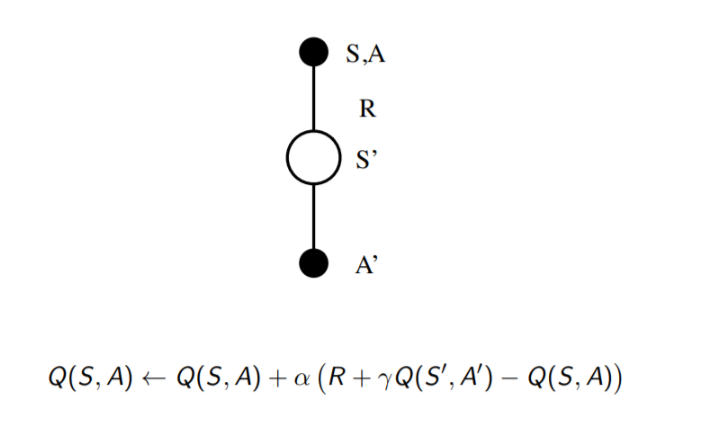
\includegraphics[width = \textwidth, height=7cm]{images/sarsa.png}
\end{center}
\item That means now I do a policy evaluation with Sarsa and after each evaluation I do a policy update(ex. with epsilon greedy). 
Here the algorithm: 
\begin{center}
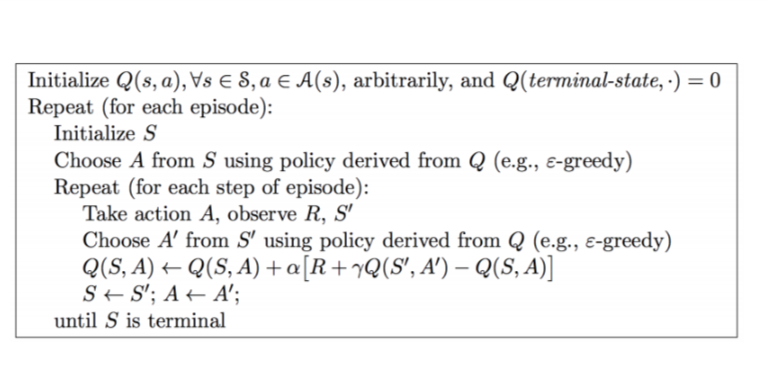
\includegraphics[width = \textwidth, height=7cm]{images/sarsa_algo.png}
\end{center}
\item Sarsa is an on-policy algorithm. 
\item We can  also do n-step Sarsa, where we look at several rewards and then look at the q-value. If we look at all rewards from the whole episode, we have MC. $$ Q(S_t, A_t) = Q(S_t, A_t) + \alpha (q_t^{(n)} - Q(S_t,A_t))$$ with the n-step Q-return $$q_t^{(n)} = R_{t+1} + \gamma R_{t+2} + ... + \gamma^{n-1} R_{t+n} + \gamma^n Q(S_{t+n})$$
\item There is also a forward View Sarsa($\lambda$). The $q^{\lambda}$ return combines all n-step Q-returns $q_t^{(n)}$, using weight $(1-\lambda)\lambda^{n-1}$: $$q_t^{\lambda} = (1-\lamda) \sum_{n=1}^{\infty} \lambda^{n-1}q_t^{(n)}$$.
\newline
Forward-view Sarsa($\lambda$):
$$Q(S_t, A_t) = Q(S_t, A_t) + \alpha (q_t^{\lambda} - Q(S_t,A_t))$$
\item Remember there is also a backward view, because the problem of the forward view is that we do not have an online algorithm. We need to wait until the end of an episode to update a current state. Just like in TD(lambda) we use eligibility traces in an online algorithm. But Sarsa(lambda) has one eligibility trace for each state-action pair: $$E_0(s,a) = 0$$ $$ E_t(s,a) = \gamma \lambda  E_{t-1}(s,a) + 1(S_t = s, A_t = a)$$ \newline
So When we visit a state action pair, we increment it. And all the states that we do not visit we decay a little bit, until we visit them again. Q(s,a) is updated for every state s and action a in proportion to TD-error $\delta_t$ and eligibility trace $E_t(s,a)$: 
$$ \delta_t = R_{t+1} + \gamma Q(S_{t+1}, A_{t+1}) - Q(S_t, A_t)$$ $$Q(s,a) = Q(s,a) + \alpha \delta_t E_t(s,a)$$


\begin{center}
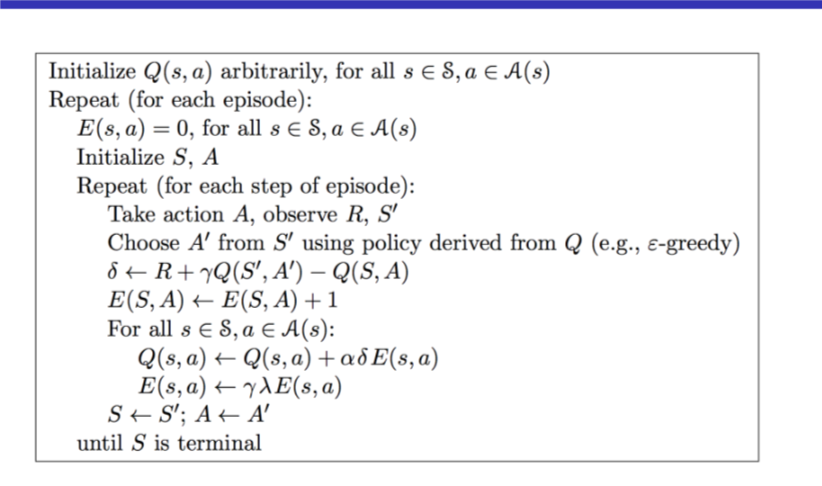
\includegraphics[width = \textwidth, height=7cm]{images/sarsa_lambda.png}
\end{center}

\item What is the difference between Sarsa(0) and Sarsa(lambda)? When you are in a grid world and you have a random walk which eventually leads you to some gold, with Sarsa(0) you only update the value of the second last state(just before the gold). Because you thought you would get a reward of 0 but actually got a reward of 1. All other states remain at value 0. If you now would take the exact same path again, the state of 1 is propagated back a little bit more. For Sarsa(lambda) with an Eligibility trace you increase all the states of the path according to the weight of the eligibility trace, i.e. the last steps get more update than the first ones. Note if lambda is equal to 1 we have the same as MC, because all the old states are not decayed. 
\item If we look at it with the forward view, you look at a state and you have to wait until the end of the episode. And for each state you look at the one-step return, two-step return, which all would yield nothing. Except the n-step return which would give you something, but which would be weighted such that the actual update would be exactly the same as with the eligibility trace backward view(there we also have a weighting with the eligibility trace). But the backward view is much more efficient.  
\end{itemize}

\subsection{Off- Policy Learning/Q-learning}
\begin{itemize}
    \item evaluate target policy $\pi(a|s)$ to compute $v_{\pi}(s)$ or $q_{\pi}(s,a)$, while following behaviour policy $\mu(a|s)$. Why would we want to do this? Because we want to learn from observing humans or other agents. We also mgiht want to re-use experience generated from old policies. Or we might want to learn about optimal policy while following an exploratory policy. Or finally we might want to learn about multiple policies while following one policy. 
    \item Importance sampling: Estimate the expectation of a different distribution. $$ E_{X~P}[f(X)] = \sum P(X)f(x) = \sum Q(x) \frac{P(x)}{Q(x)} f(x) = E_{X~Q}[\frac{P(X)}{Q(x)}f(X)]$$
    \item We can apply importance sampling to Monte-Carlo learning by using returns generated from $\mu$ to evaluate $\pi$. Weight return $G_t$ according to similarity between policies. Multiply importance sampling corrections along whole episode $$G_t^{\pi/mu} =\frac{\pi(A_t|S_t)\pi(A_{t+1}|S_{t+1})}{\mu(A_t|S_t) \mu(A_{t+1}|S_{t+1}}...\frac{\pi(A_T|S_T}{\mu(A_T|S_T)}G_t$$ Update value towards corrected return: $$V(S_t) = V(S_t) + \alpha(G_t^{\pi/\mu}-V(S_t))$$
    \newline In practice this is useless as it has a very high variance. 
    \item So we need to use TD learning and Bootstrap. So now we only do importance sampling over one step. WE weigh TD target $R + \gamma v(S')$ by importance sampling and thus only need one sampling correction: $$ V(S_t) = V(S_t) + \alpha (\frac{\pi(A_T|S_t)}{\mu(A_t|S_t}(r_{t+1} + \gamma V(S_{t+1})) - V(S_t)$$
    \item The policy which works best for off-policy learning is Q-Learning. Here no importance sampling is required. The next action is chosen using behaviour policy $A_{t+1} ~ \mu(.|S_t)$. But we consider alternative successor action $A' ~ \pi(.|S_t)$ and update $Q(S_t, A_t)$ towards value of alternative action. $$Q(S_t, A_t) = Q(S_t,A_t) + \alpha(R_{t+1} + \gamma q(S_{t+1}, a') - Q(S_t, A_t)$$
    \item When we talk about Q-learning(SARSAMAX), one usually means the following special case. We no allow both behaviour and target policies to improve. The target policy $\pi$ is greedy w.r.t Q(s,a) $$\pi(S_{t+1} = argmax_{a'}Q(S_{t+1},a')$$ The behaviour policy $\mu$ is e.g. epsilon-greedy w.r.t Q(S,a). 
    \newline The Q-learning target then simplifies: 
    $$R_t + \gamma Q(S_{t+1}, A')$$
    $$R_{t+1} + \gamma Q(S_{t+1}, argmax_{a'}Q(S_{t+1}, a'))$$ $$= R_{t+1} + max_{a'} \gamma q(S_{t+1}, a')$$
\begin{center}
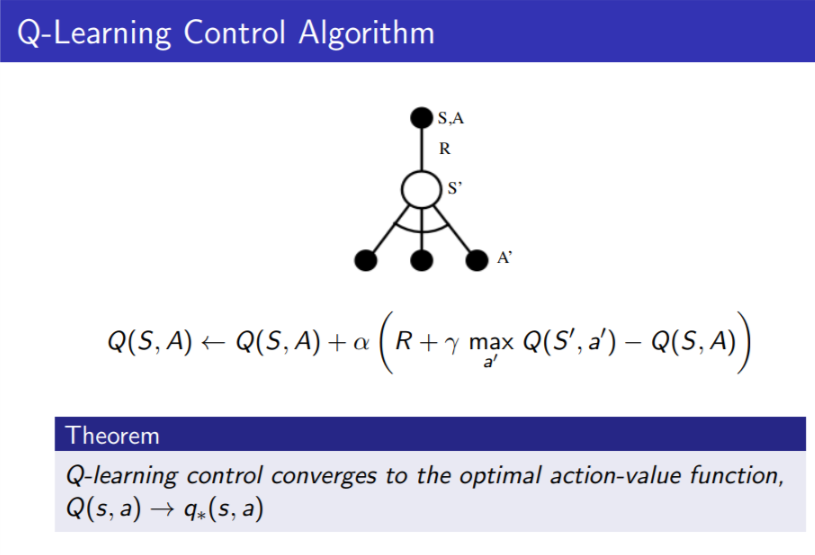
\includegraphics[width = \textwidth, height=7cm]{images/qlearning.png}
\end{center}
\begin{center}
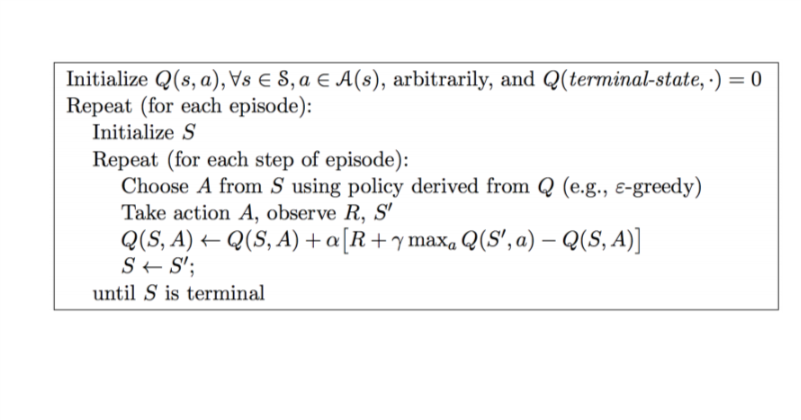
\includegraphics[width = \textwidth, height=7cm]{images/qlearningalgo.png}
\end{center}
\begin{center}
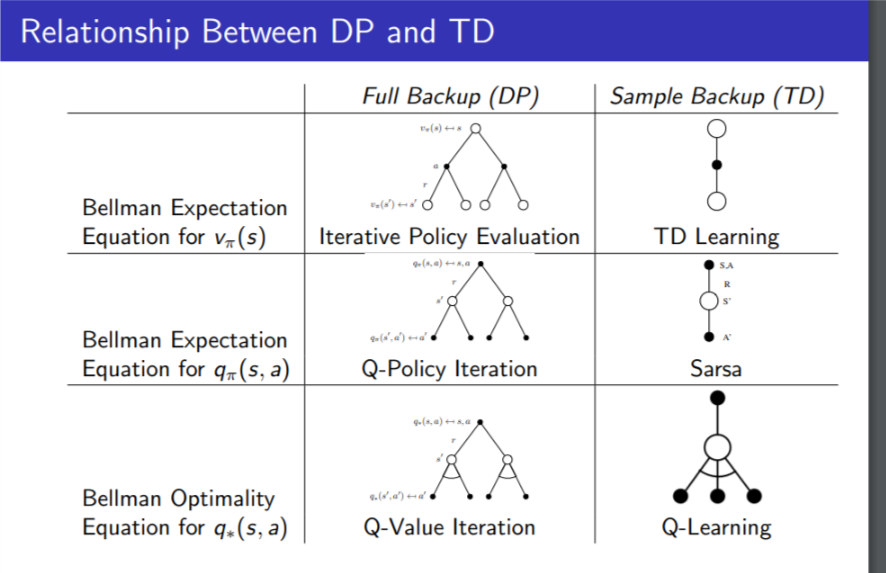
\includegraphics[width = \textwidth, height=7cm]{images/summary1.png}
\end{center}
\begin{center}
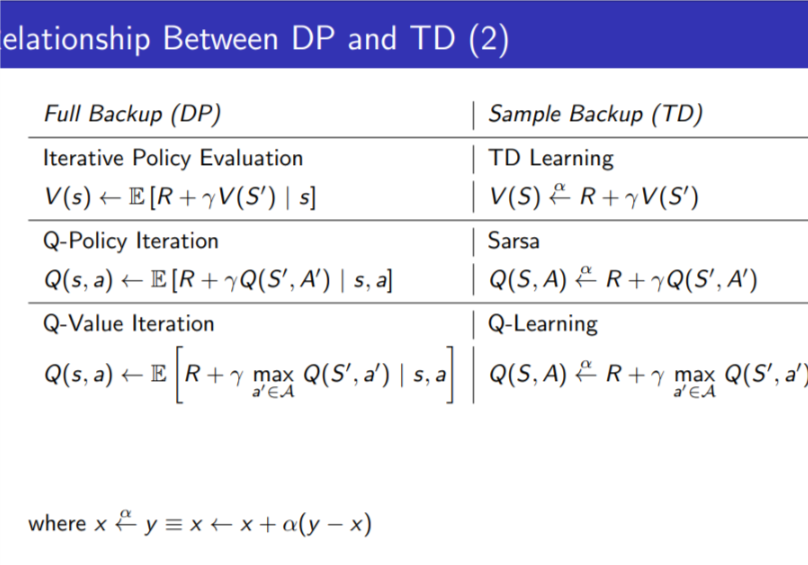
\includegraphics[width = \textwidth, height=7cm]{images/summary2.png}
\end{center}
\end{itemize}

\section{Value Function Approximation}
\begin{itemize}
    \item Today we will look at incremental methods and batch methods. With incremental methods you take a function approximator(like a NN) and incrementally every single step you see a new piece of data that comes in and immediately online you take some step to update your value function online. Batch methods look at everything you have seen so far and update the value function accordingly. 
\subsection{Incremental Methods}
    \item The problem with real problems is that they might get arbitrarily large and we cannot just build a table anymore. Also we want to be able to generalize to different settings. So today we are going to look at how to compute value functions. 
    \item So again we want to scale up prediction and control. 
    \item So far we have represented value functions by a lookup table, i.e. every state or every state-action pair has an entry V(s) or Q(s,a). For control we need to be able to pick our actions without having a model(so we used Q(s,a). The problem with large MDP's is that there are too many states and/or actions to store in memory but also it is to slow to learn the value of each state individually.
    \item The solution to that is function approximation: 
    $$v'(s,w) \approx v_{\pi}(s) $$ or $$ q'(s,a,w) \approx q_{\pi}(s,a)$$ Note that our approximation works for any state s, even if we have not seen it yet. W are weights. This allows us to generalize to unseen states. We can update the parameters w using MC or TD learning. \item With value functions we can use different types of function approximators. You feed in your state s and can get $v'(s,w)$. You can feed in s and a and get $q'(s,a,w)$. We can also feed in a state s and get $q'(s,a_1,w)...q'(s,a_m,w)$
    \item There are a lot of different function approximators such as linear combinations of features, Neural Net's, Decision trees, Nearest Neighbours, Fourier/Wavelet based etc. We will focus on differential function approximators such as Linear combinations of features and Neural networks. Here its easy to update the weights with the gradient we can calculate. 
    \newline
    Furthermore, we require a training method that is suitable for non-stationary, non-iid data. Because the value function we try to approximate always changes depending on our changing policy and the rewards. It is non-iid because where I am now is very highly correlated to where I am going to be next. 
    \item Lets have a look at SGD: 
    \begin{center}
    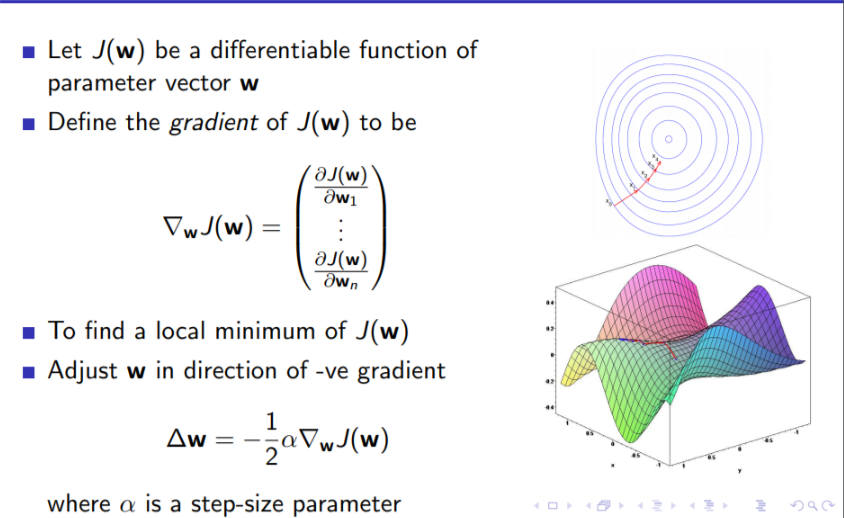
\includegraphics[width = \textwidth, height=7cm]{images/sgd.png}
    \end{center}
    
    \begin{center}
    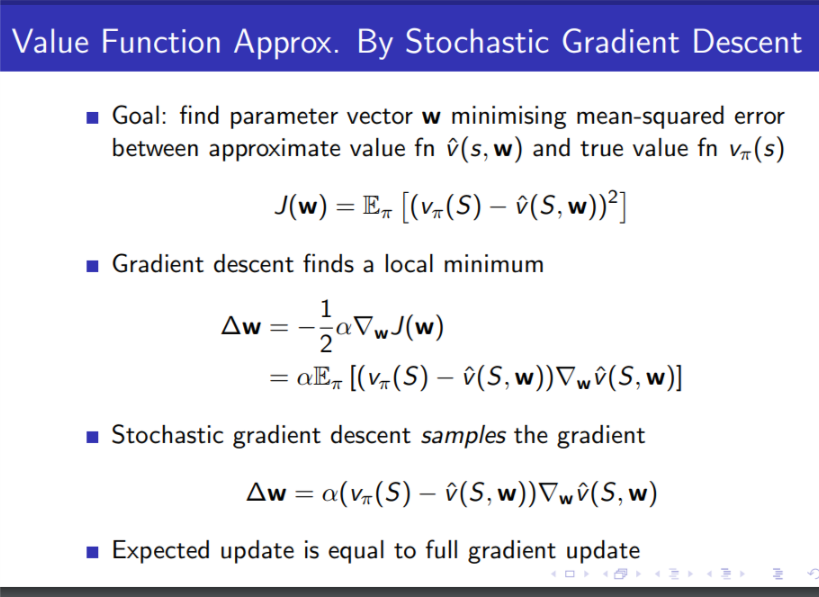
\includegraphics[width = \textwidth, height=7cm]{images/value_sgd.png}
    \end{center}
    Remember that the expectation is just averaging. 
    \item So the idea is that we sample a state and then we compare our estimate for our value function with a true(oracle) value function. How can we do it without having the oracle knowledge?
    \item we often represent a state by a feature vector, for example the distance of a robot to landmarks or trends in the stock market etc. 
    \item How does Linear Value Function approximation works? The idea is to use some weights and to use some state-feature instead of just a state. The nice thing is also that you only multiply by the state-features that are actually active. So for example if you don't have a queen, you won't multiply by the "queen-feature" of the state, because it is 0. 
    \begin{center}
    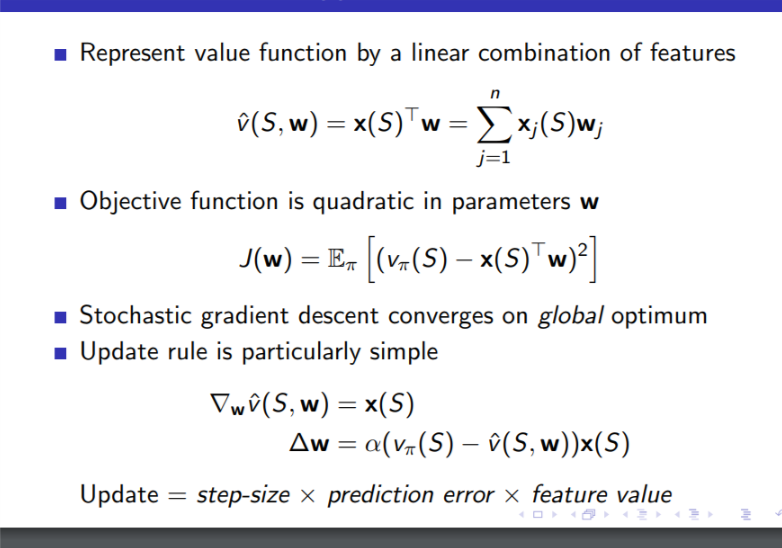
\includegraphics[width = \textwidth, height=7cm]{images/linval.png}
    \end{center}
    \item The connection to last week is that table lookup is a special case of linear value function approximation using table lookup features: 
     \begin{center}
    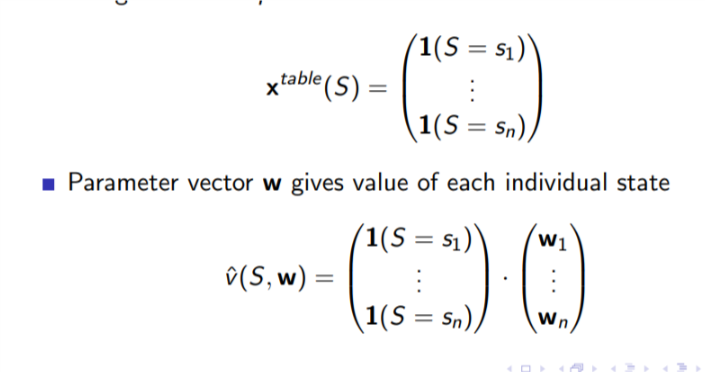
\includegraphics[width = \textwidth]{images/featuretable.png}
    \end{center}
    \item Obviously we cheated, because we do not have an oracle true value function. But we can estimate the value function $v_{\pi}$. 
     \begin{center}
    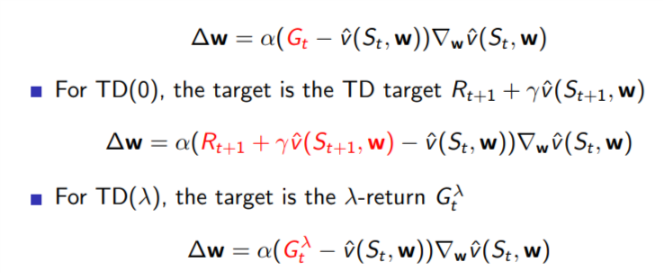
\includegraphics[width = \textwidth]{images/approx.png}
    \end{center}
    
    \item Monte-Carlo with Value Function approximation: Return $G_t$ is an unbiased, noisy sample of the true value $v_{\pi}(S_t)$. We can therefore apply supervised learning to the training data that we generate: 
    $$<S_1,G_1>, <S_2,G_2>, ...<S_T,G_T>$$
    \item The TD-target $R_{t+1} + \gamma v'(S_{t+1},w)$ is a biased sample of the true value $v_{\pi}$. Here one can also build a data set and apply supervised learning on: 
    $$<S_1,R_2 + \gamma v'(S_2,w)>, <S_2, R_3 + \gamma v'(S_3,w)>, ...$$
    \item Remember that for the $TD(lambda)$ we can use a forward or backward view. The dataset looks like: 
    $$<S_1, G_1^{\lambda}>, <S_2, G_2^{\lambda}> ...$$
    Forward view linear TD(lambda): 
    $$\Delta w = \alpha(G_t^{\lambda} - v'(S_t, w))\nabla_w v'(S_t,w)$$
    $$= \alpha(G_t^{\lambda} - v'(S_t,w))x(S_t)$$
    Backward view: $$\delta_t = R_{t+1} + \gamma v'(S_{t+1},w) - v'(S_t,w)$$
    $$E_t = \gamma \lambda E_{t-1} + x(S_t) $$
    $$\Delta w = \alpha \delta_t E_t$$
    \item How can we do Control with Value Function approximation? We are going to start with some weights and we start with some epsilon greedy policy. So we do: \newline 
    Policy evaluation: Approximate policy evaluation $q'(.,.,w) \approx q_{\pi}$
    \newline Policy improvement: epsilon-greedy policy improvement. 
    \item 
    \begin{center}
    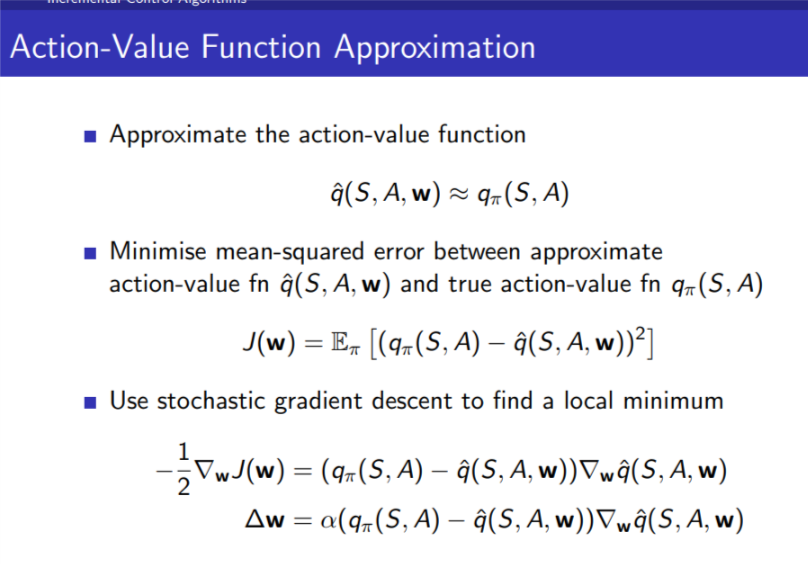
\includegraphics[width = \textwidth]{images/actionvalue approx.png}
    \end{center}
    Note that from there on we can do the same steps as before, use linear state-action feature vectors, TD(0), MC, TD(lambda) etc. 
    \item Sometimes we should not use TD, because it could diverge. 
    \begin{center}
    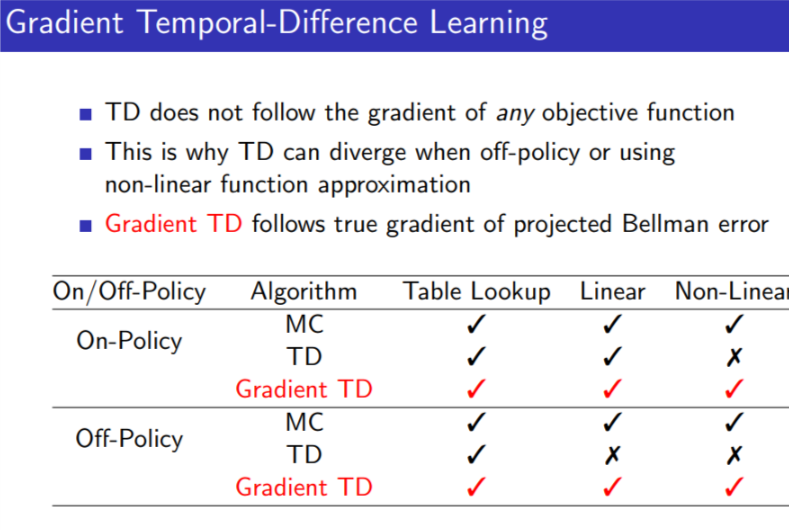
\includegraphics[width = \textwidth]{images/tdconvergence.png}
    \end{center}
    \item Convergence of Control Algorithms: 
    \begin{center}
    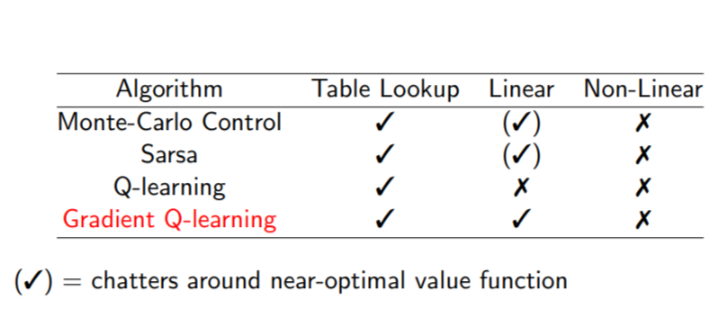
\includegraphics[width = \textwidth]{images/controlconvergence.png}
    \end{center}
    Chatter means that we take steps towards the goal, and then again we move away from the goal. And like that we kind of not get closer to the real goal. 
\end{itemize}

\subsection{Batch methods}
\begin{itemize}
    \item Gradient descent is simple and appealing but it is not very sample efficient. Batch methods seek to find the best fitting value function given the agent's (whole) experience(training data). 
    \item Given value function approximation $ v'(s,w) \approx v_{\pi}(s)$ and experience D consisting of <state, value> pairs(assuming we again have an oracle): $$D 0 {<s_1,v_1^{\pi}>, <s_2,v_2^{\pi},...}$$ Which parameters w give the best fitting value function v'(s,w)? Least squares algorithm finds parameter vector w minimizing sum-squared error between our estimate of $v'(s_t,w)$ and the target values $v_t^{\pi}$. 
    $$ LS(w) = \sum_{t=1}^T (V_t^{\pi}j- v'(s_t,w))^2$$
    $$ E_D[(v^{\pi} - v'(s,w))^2]$$
    Note, before we always looked at one specific state which we were at in a specific timestep. Now we look at the whole data. There is an easy way to find the solution, its called experience replay.
    \newline
    1. Sample state, value from experience $<s,v^{\pi}$ from D
    2. Do stochastic gradient descent update: 
    $$ \Delta w = \alpha(v^{\pi} - v'(s,w)) \nabla_w v'(s,w)$$
    So note that here everything is decorrelated as we sample from it in a random fashion. The idea is also that you keep going over your data and squeze out everything you can from it, instead of throwing it away after one step. 
    \item Deep Q-Networks: It uses experience replay and fixed Q-targets. Take action $a_t$ according to epsilon reedy policy. We then store a transition $(s_t, a_t, r_{t+1}, s_{t+1}$ in replay memory D. We then sample a random mini-batch of transitions (s,a,r,s') form D and compute Q-learning targets w.r.t. old, fixed parameters$w^-$. We the optimize MSE between Q-networks and Q-learning targets: $$
    L_i(W_i) = E_{s,a,r,s' ~ D_i}[(r + \gamma max_{a'} Q(s',a',w_i^-) - Q(s,a,w_i))^2]$$
    We use a variant of SGD. 
    \newline 
    Note that we have a giant NN which approximates Q. So the idea is that instead of having q-value from an oracle, you have an estimate of those from Q-learning(instead of SARSA as before) and we then approximate these.
    \item IMPORTANT NOTE: There is a key thing I missed until now. Remember, we estimate the value of a state for example with SARSA and then try to approximate this estimate with a Neural Net. Well this state value is computed as $R_{t+1} + \gamma v'(S_t,w)$. So we actually see one reward. But the estimate of the value of the next state is not calculated by trying every action or something similar, for the estimate of the next state we actually use our Neural Network that we are currently training with the old weights it had. 
    \item Note that this algorithm is stable. Why? Because we do experience replay, i.e. we decorrelate our data. The second idea is that we keep two different Neural Net's with different parameters. We have our estimate of the state action value which is calculated with Q-learning. But if you look above, this gives us a reward plus the state-action value of the next state. This state-action value of the next state is computed with our Neural Network which tries to approximate the estimate of our state-action value. And now while we try to calculate the gradient of the weights, we use the old Networks with old weights to approximate the state-action value of the next state. These old weights are fixed and only updated ex. every 1000 steps. 
    \item For the Atari game, They did end-to-end learning  of values Q(s,a) from pixels s. The Input state s was a stack of raw pixels from the last 4 frames. The output Q(s,a) for 18 joystick/button positions. The rewards is change in score for that step. 
    \item Experience replay finds least squares solution but it may take many iterations. Using linear value function approximation we can solve the least squares solution directly. 
\end{itemize}



\section{Policy Gradient Methods}
\begin{itemize}
    \item Today we will look at methods which optimize the policy directly. So today we will look at finite difference Policy Gradient, Monte-Carlo Policy Gradient and Actor Critic policy gradient. Last week we tried to estimate the action-value or value function. The policy was then generated directly from the value function using epsilon greedy. In this lecture we will directly parametrize the policy $$\pi_0(s,a) = P(a|s,a\theta)$$
    We will again focus on model-free reinforcement learning. 
    \item The reason we do this function approximation is because we want to be able to scale to large, complicated MDP's. Where sometimes it is not possible for each distinct state to say I need to take this action or this action. That's why we need to do function approximation. 
     \begin{center}
    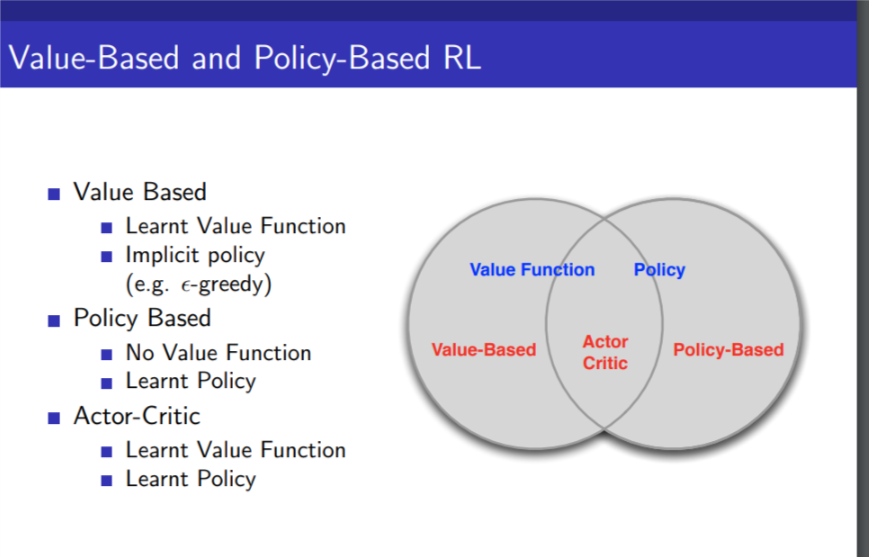
\includegraphics[width = \textwidth]{images/algorithm_overview.png}
    \end{center}
    \item What are some advantages of Policy Based RL? In some situations it is more efficient to store the policy instead of the value function. Better convergence properties and it is effective in high-dimensional or continuous action spaces(We do not have to compute a max). Also it can learn stochastic policies. 
    \newline 
    Disadvantages: Typically it converges to a local rather than a global optimum. Evaluating a policy is typically inefficient and high variance. 
    \item  Why would we want a stochastic policy? Consider a two-player game of rock-paper-scissors. A deterministic policy can easily exploited. 
    \item Also if we are in a partially observed MDP(i.e. we do not know all the transitions etc.), a deterministic policy might be bad. See this example: 
      \begin{center}
    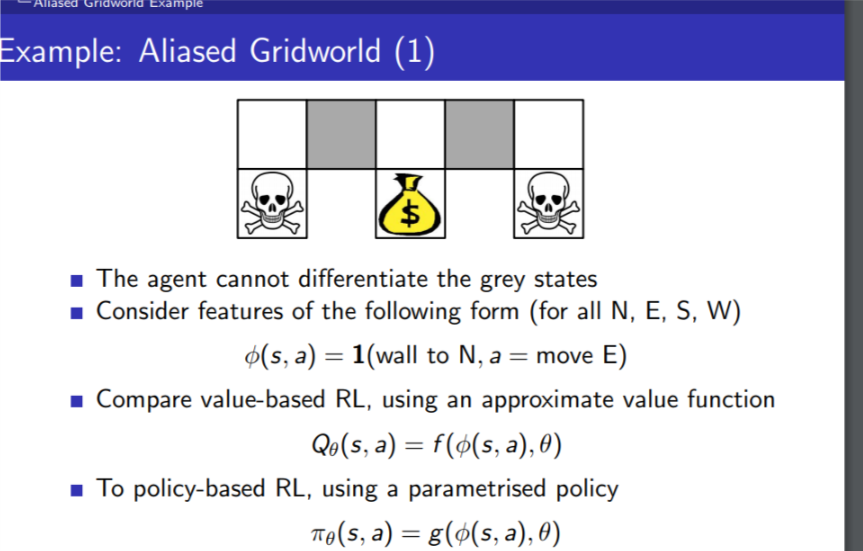
\includegraphics[width = \textwidth]{images/ex1.png}
    \end{center}
      \begin{center}
    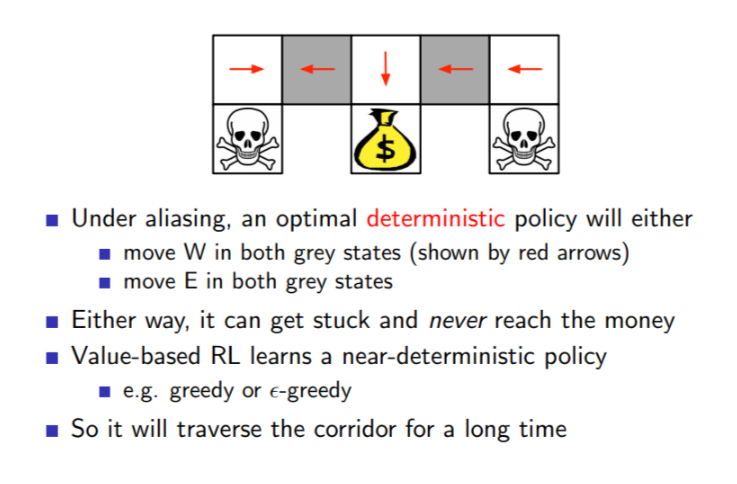
\includegraphics[width = \textwidth]{images/ex2.png}
    \end{center}
      \begin{center}
    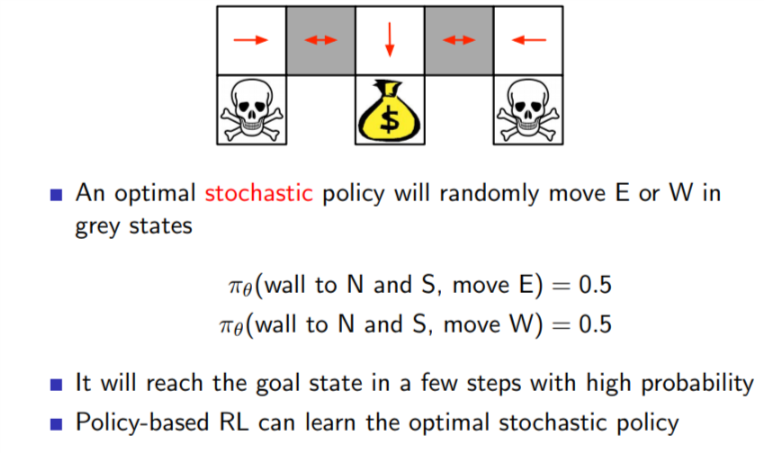
\includegraphics[width = \textwidth]{images/ex.png}
    \end{center}
    \item There are different objective Functions. 

      \begin{center}
    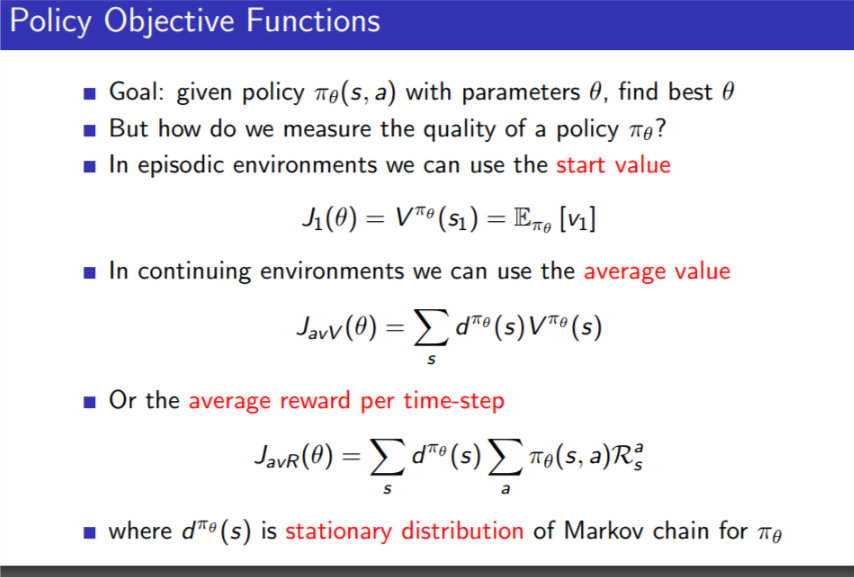
\includegraphics[width = \textwidth]{images/policy_goals.png}
    \end{center}
    Fortunately for us the same methods apply to all three objectives. The only thing that differs is th distribution that I am in some state s. 
    \item Now we want to optimize the policies(i.e. the theta). So find $\theta$ that maximizes $J(\theta)$. Some approaches do not use gradient such as Hill climbing, Simplex or Genetic algorithms. Greater efficiency is often possible using gradients such as gradient descent, conjugate gradient or quasi-newton. We focus on gradient descent. 
    \end{itemize}

    
\subsection{Finite Difference Policy Gradient}
\begin{itemize}
    \item We have an objective function and we try to search for a maximization of this function. Thus we want to do gradient ascent. 
    \item A very naive approach to evaluate policy gradient of $\pi_0(s,a)$ is to just perturb our parameters $\theta$ by a small amount epsilon in the k-th dimension(to estimate k-th partial derivative). We do this then for each dimension(which is ineffective). But this works for arbitrary policies, even if the policy is not differentiable.
    $$\frac{\partial J(\theta)}{\partial \theta_k} \approx \frac{J(\theta + \epsilon u_k - J(\theta)}{\epsilon}$$
    \item We now compute the policy gradient analytically. Assume the policy is differentiable whenever it is non-zero and we know the gradient $\nabla \pi_0(s,a)$.Likelihood ratios exploit the following identity of the log: $$\nabla_{\theta} \pi_{\theta}(s,a) = \pi_{\theta}(s,a) \frac{\nabla_{\theta} \pi_{\theta}(s,a)}{\pi_{\theta}(s,a)}$$ 
    $$ = \pi_{\theta}(s,a) \nabla_{\theta} log \pi_{\theta}(s,a)$$
    Now the score function is $\nabla_{\theta}log \pi_{\theta}(s,a)$
    \item We will us a a softmax policy as a running example. It is basically something where we want to have some smoothly parametrized policy that tells us how frequently we should choose an action for each discrete set of actions. So its an alternative to epsilon-greedy etc. Weight actions using linear combination of features ¨$\phi(s,a)^T\theta$. The probability of an action is proportional to exponentiated weight:$$ \pi_{\theta}(s,a) \propto e^{\phi(s,a)^T\theta}$$
    The score function is then $$\nabla_{\theta}log \pi_{\theta}(s,a) = \phi(s,a) - E_{\pi_{\theta}}[\phi(s,.)]$$
    For example in atari, we would have some features for going left and some for going right and whichever scores higher would get higher probability when we pick these actions. We would like to calculate the gradient of this thing. Note that the gradient is just the feature minus the average feature. So if a feature occurs more than usual and gets a good reward, we want to change the policy. Note that the expectation is the normalization constant. 
    \item in continuous action spaces, a Gaussian policy is natural. The mean is a linear combination of state features $ \mu(s) = \phi(s)^T\theta$. The variance may be fixed or can also be parametrized. The policy is a Gaussian, $a\sim N(\mu(s),\sigma^2$. The score function is then $$\nabla_{\theta}log \pi_{\theta}(s,a) = \frac{(a-\mu(s))\phi(s)}{\sigma^2}$$
    \subsection{Monte Carlo Policy Gradient/REINFORCE}
    \item Our goal is to maximize our reward. So to maximize our expected reward, we need to move in the direction of our score-function times our reward. If you have positive or negative reward you move into opposite directions. 
     \begin{center}
    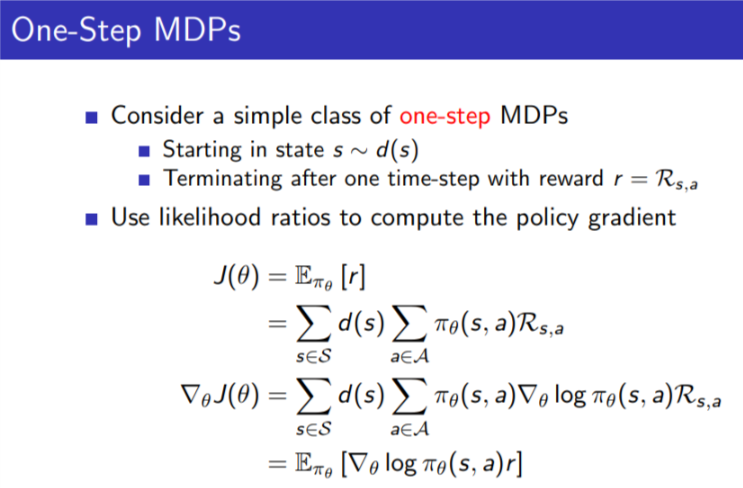
\includegraphics[width = \textwidth]{images/onestep.png}
    \end{center}
    \item What do we do, if we want to apply this trick not only to one step MDP's but to multiple steps. We have to replace the instantaneous reward r with a long-term value. $Q^{\pi}(s,a)$
     \begin{center}
    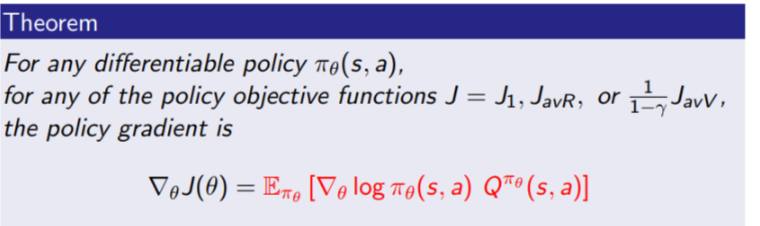
\includegraphics[width = \textwidth]{images/policygrad.png}
    \end{center}
    \item REINFORCE/ Monte-Carlo Policy Gradient: 
      \begin{center}
    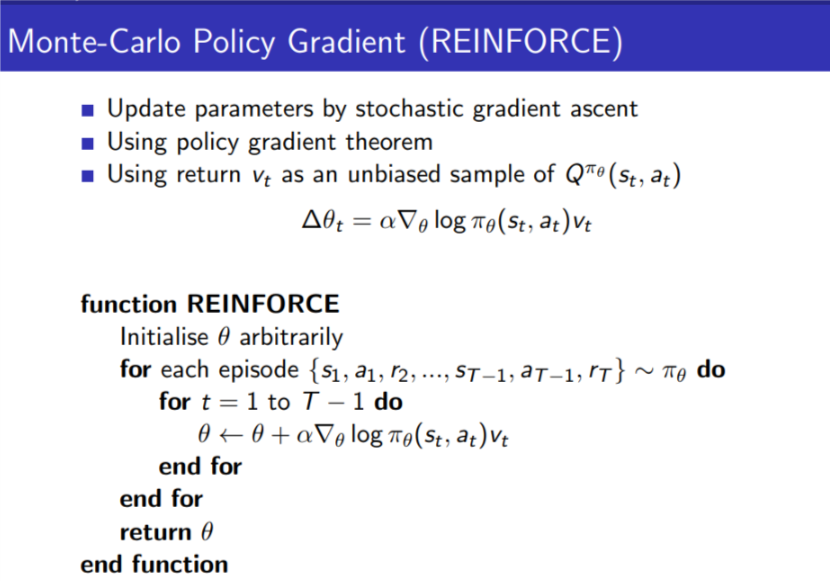
\includegraphics[width = \textwidth]{images/reinforce.png}
    \end{center}
    That means we are in a state, we take an action and see what rewards we get from there on wards and use this as an estimate of Q. So we basically sample a whole episode. 
    \item With this method we can see that the learning curve is very smooth, but also very slow. So in the rest of this class we will try to make it more efficient. 
\end{itemize}¨

\subsection{Actor Critic Methods}
\begin{itemize}
    \item Monte-Carlo policy gradient still has high variance. We use a critic to estimate the action-value function, $$Q_w(s,a) \sim Q^{\pi_{\theta}}$$
    \item actor-critic algorithms maintain two sets of parameters: The critic which updates action-value function parameters w and the actor which updates policy parameters $\theta$ in direction suggested by the critic. 
    \item actor-critic algorithms follow an approximate policy gradient: $$\nabla_{\theta} J(\theta) \sim E_{\pi_{\theta}}[\nabla_{\theta}log \pi_{\theta}(s,a) Q_w(s,a)]$$
    $$\Delta \theta = \alpha \nabla_{\theta} log \pi_{\theta}(s,a) W_w(s,a)$$
    \item The critic is solving a familiar problem: policy evaluation. So how good is a policy for the current parameters. This problem was explored in previous lectures with Monte-Carlo policy evaluation, TD learning or TD(lambda). But note, we need algorithms which solve the prediction, not the control(Q-learning) problem. 
      \begin{center}
    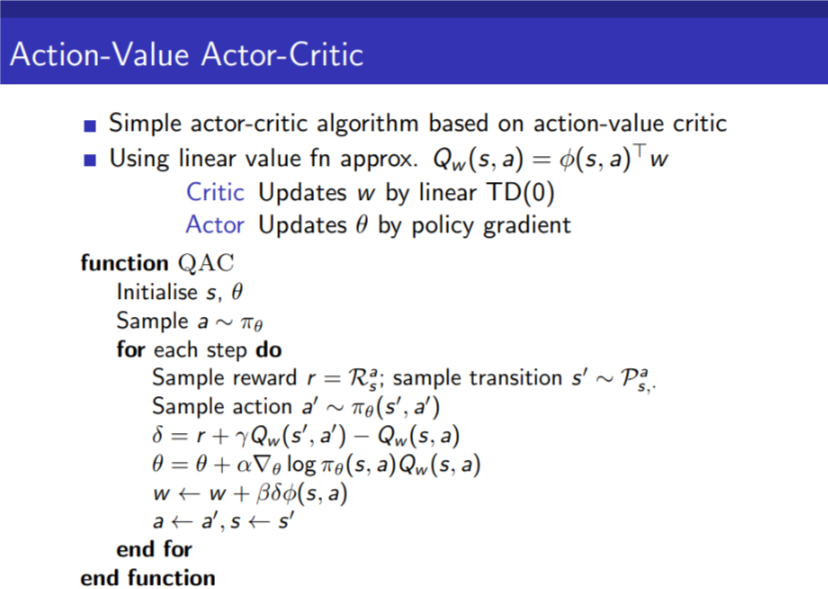
\includegraphics[width = \textwidth]{images/actorcritic.png}
    \end{center}
    \item So the difference between Policy iteration and actor critic, is that here we do not do greedy policy update but we follow the policy gradient.
    \item approximating the policy gradient introduces bias. A biased policy gradient may not find the right solution. Luckily if we choose value function approximation carefully, we can avoid introducing any bias.  
    \item There are several tricks to reduce the variance. 
      \begin{center}
    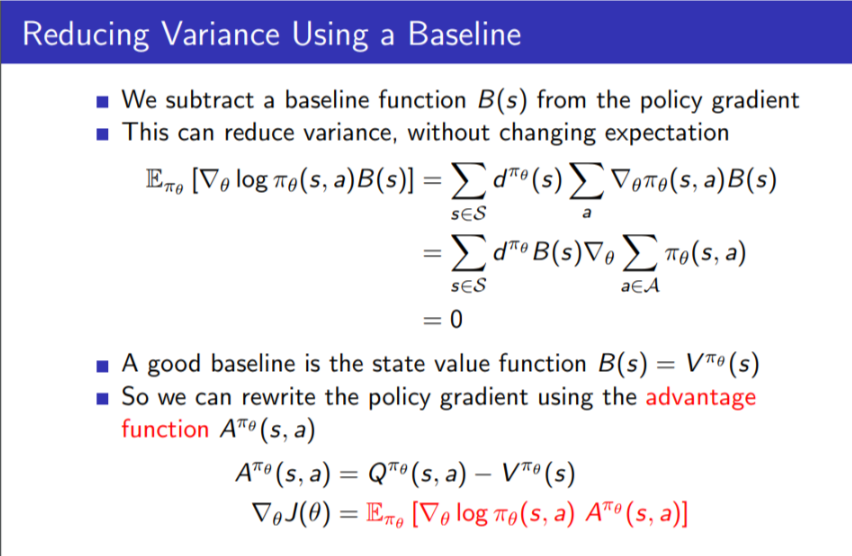
\includegraphics[width = \textwidth]{images/variance.png}
    \end{center}
    We see that adding the B(s) term does not change the Expectation. The state advantage function tells us how much better is it than usual to take action a. 
    \item The advantage function can significantly reduce variance of policy gradient method. So the critic shoudl really estimate the advantage function. For example by estimating both $V^{\pi_{\theta}} $ and $Q^{\pi_{\theta}}(s,a)$. using two function approximators and two parameter vectors: $$V_v(s) \sim V^{\pi_{\theta}}(s)$$
    $$Q_w(s,a) \sim Q^{\pi_{\theta}}(s,a)$$
    $$A(s,a) = Q_w(s,a) - V_v(s)$$ 
    And update both value functions by e.g. TD learning. 
    \item But there is an easier way: 
      \begin{center}
    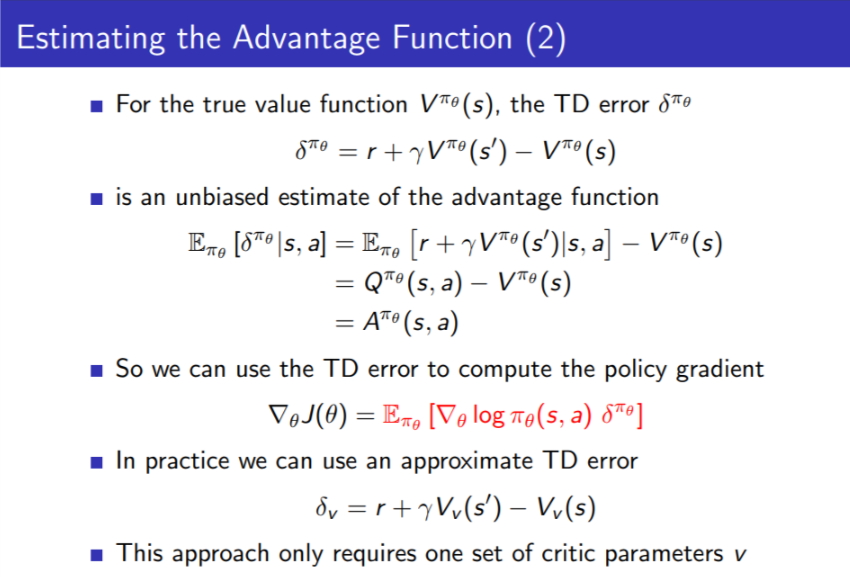
\includegraphics[width = \textwidth]{images/advantage.png}
    \end{center}
    The advantage of that is that we only need to estimate V and not also Q. 
    \item a critic can estimate value function from many targets at different time-scales. So we had MC, TD(0) and forward or backward TD(lambda). So first of all we can apply that to our critic, any evaluation algo is valid for the critic. 
      \begin{center}
    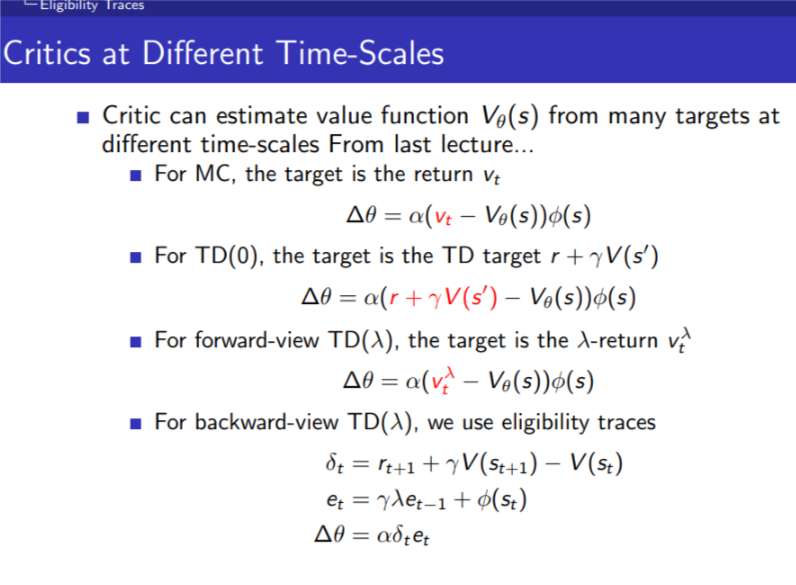
\includegraphics[width = \textwidth]{images/time.png}
    \end{center}
    But we can also apply these tricks to the actor. 
      \begin{center}
    \includegraphics[width = \textwidth]{images/actortime.png}
        \end{center}

    The MC actor policy has low bias but high variance. The TD has high bias, low variance. To have the best of both world, we use Eligibility traces. 
    
       \begin{center}
    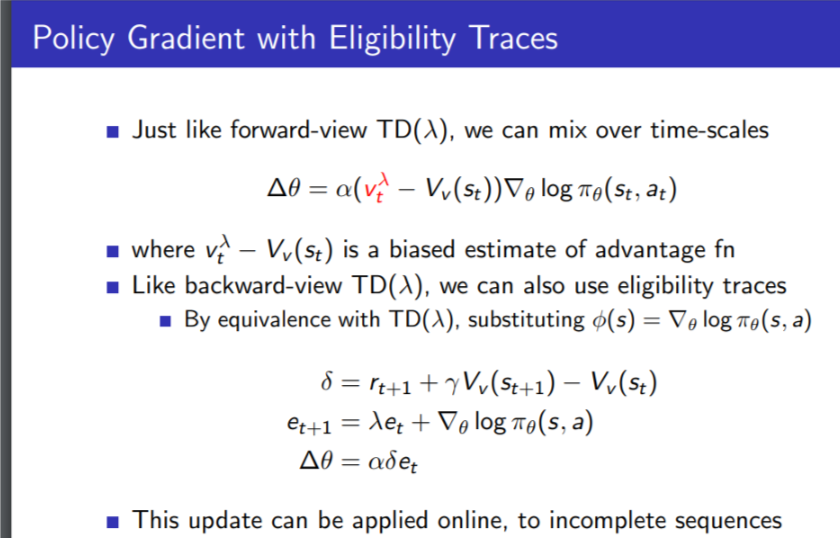
\includegraphics[width = \textwidth]{images/actorelig.png}
        \end{center}
    \item There is an important question in actor critic algorithms. Gradient ascent algorithms can follow any ascent direction A good ascent direction can significantly speed convergence. Also a policy can often be reparametrized without changing action probabilities. For example increasing score of all actions in a softmax policy. The vanilla gradient is sensitive to these reparametrizations.  So in spite the fact that we approximate the true value function, we can still find the true value function. 
    \item Here a summary: 
       \begin{center}
    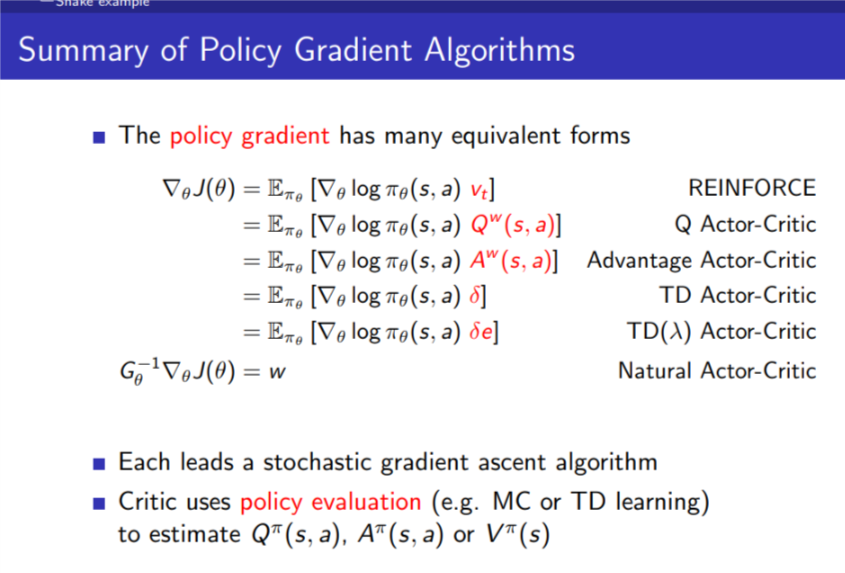
\includegraphics[width = \textwidth]{images/summaryactor.png}
        \end{center}
\end{itemize}

\section{Integrating Learning and Planning}
\begin{itemize}
    \item We will have a look at model-based RL, Integrated architectures and simulation-Based Search. In Model Based RL we will especially see how one can plan better by having a model. Integrated architectures give us the best of both worlds, model based and no model RL. 
    \item Before we looked at learning a policy or a value function directly from experience. Today we try to learn a model directly from experience and use planning to construct a value function or policy. 
    \item A model in our context is an idea of an MDP. 
    \item Model-Free RL: NO model, we learn a value function from experience. Model based RL means that we learn a model from experience and plan a value function (and/or policy) form the model. 
    \end{itemize}

    \subsection{Model Based RL}
    \begin{itemize}
        \item We have a value/policy on which we act to gather experience. From that we learn a model and then plan on this model to learn the value/policy. 
        \item Advantages: Can efficiently learn model by supervised learning methods and can reason about model uncertainty. For example in chess, we can have the rules of the game as a model which allows us to do a tree search of the next steps. 
        \item Disadvantages: First learn a model, then construct a value function which introduces two sources of approximation error. 
        \item What is a mode? It is a representation of an MDP <S,A,P,R> parametrized by $\eta$. We will assume that state space S and action space A are known. So a model $M = <P_{\eta}, R_{\eta}>$ represents  state transitions $P_n \sim P$ and rewards $R_n \sim R$: 
        $$S_{t+1} \sim P_n(S_{t+1}| S_t, A_t)$$
        $$R_{t+1} = R_n(R_{t+1}| s_t, A_t)$$
        Typically we assume conditional independence between state transitions and rewards. 
        \item For chess for example the model learning would be to learn the rules of the game. Given the rules we want to plan. 
        \item Goal is to estimate the model $M_n$ from experience $S_1, A_1, R_2$ etc. This is a supervised learning problem, because we have a dataset which tells us that if we are in $S_1, A_1$ we will get $R_2$ and land in $S_2$. 
        \item So learning the reward from a state action pair is a regression problem and learning the next state from a state action pair is a density estimation problem.  The loss function can be MSE(regression) and for the second we could take KL-divergence. We want to find $\eta$ to minimize the empirical loss. 
        \item Note that often the state space is not given or we might want to learn state features. 
        \item We will look at the table lookup model in which we  have a state and an action and try to predict the reward and next state seperately. Then there are also linear expectation models, linear gaussian models, gaussian process models, Deep Belief Netowrk Model. 
        \item The model is an explicit MDP, P', R'. We count visits N(s,a) to each state action pair:
        $$ P'_{s,s'}^a = \frac{1}{N(s,a)} \sum_{t=1}^T 1(S_t,A_t,S_{t+1} = s,a,s')$$
        $$R_s^a = \frac{1}{N(s,a)} \sum_{t=1}^T 1(S_t,A_t= s,a)R_t$$
        \newline
        Alternatively at each time-step t, we can record experience tuple. To sample model, randomly pick tuple matching <s,a,.,.>.
        \item Once we have a model we can solve it/plan with our favourite planning algorithm such as value iteration, policy iteration, tree search etc. 
        \item Sample based planning is also very powerful. We use the model only to generate samples, i.e. we sample experience from the model:
        $$S_{t+1} \sim P_{\eta}(S_{t+1}| S_t, A_t)$$
        $$R_{t+1} = R_{\eta}R_{t+1} | s_t, A_t$$
        and to these samples we apply model-free RL such as Monte-Carlo control, Sarsa, Q-learning etc. The advantage of this approach is that we can sample infinite data. 
        \item Given an imperfect model, we might not be able to learn anything useful. So our performance is limited to the optimal policy of approximate MDP. So the solution is that when the model is wrong we should use model-free RL or reason explicitly about our model uncertainty. 
    \end{itemize}
    \subsection{Integrated Architectures}
    \begin{itemize}
        \item We consider two sources of experience: First of all we have real experience samples from the environment(true MDP). 
        $$S' \sim P_{s,s'}^a$$
        $$R  = R_s^a$$
        And then we also have simulated experience from the model(approximate MDP):$$S' \sim P_{\eta}(S'|S,A)$$
        $$R = R_{\eta}(R|S,A)$$
        \item Dyna-Architecture. WE learn a model from real experience and learn and plan our value function (and/or policy) from real and simulated experience. That means from our experience we do direct RL and we do model learning and planning from that. 
            \begin{center}
    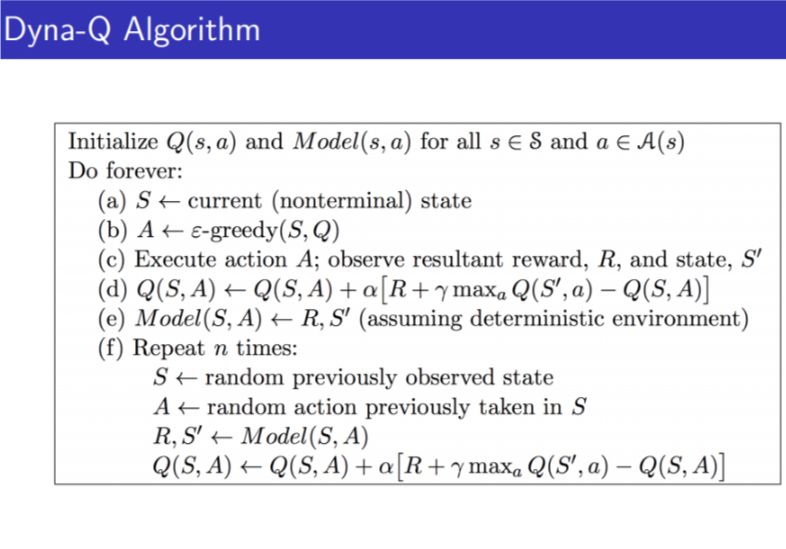
\includegraphics[width = \textwidth]{images/dyna.png}
        \end{center}
        \item We can also optimize the algorithm such that it explores more.
    \end{itemize}
\subsection{Simulation-Based Search}
\begin{itemize}
    \item Here we look the idea of taking samples from imaginary experience. We are going to use sampling and forward search.
    \îtem Forward search algorithms select the best action by lookahead. They build a search tree with the current state at the root. Using a model of the MDP to look ahead. We do not need to solve the whole MDP, we just need to solve parts of it starting from now. 
    \item Simulation based search is a forward search paradigm using sample-based planning. That means we simulate episodes of experience from now with the model. WE apply model free RL to simulated episodes. The reason why it is forward is because we always sample from the current state on. Once we get these trajectories we apply model-free RL. 
    \item We simulate episodes of experience from now with the model: $${s_t^k, A-t^k, r_{t+1}^k,....,S_T^k} \sim M_v$$
    Note that we apply for example Monte-Carlo control which is then called Monte Carlo search, or if we apply Sarsa it is called TD search. 
    \item MOnte-Carlo Search: Given a model $M_v$ and a simulation policy $\pi$, for each action we simulate K episodes from current(real) state $s_t$: $${s_t, a, r_{t+1}^k, A_{t+1}^k, ..., S_T^k}_{k=1}^K \sim M_{v,\pi}$$
    We then evaluate the actions by the mean return(Monte-Carlo evaluation): $$Q(s_t, a) = \frac{1}{k} \sum_{k=1}^K G_t -> q_{\pi}(s_t,a)$$
    We select the current(real) action with maximum value: 
    $$a_t = argmax_{a \epsilon a}Q(s_t,a)$$
    \newline
    So for example if I can go left, I simulate 100 times going left and take the average empirical expected reward. 
    \item Here is another thing that works nicely in practice(Alpha GO).     \begin{center}
    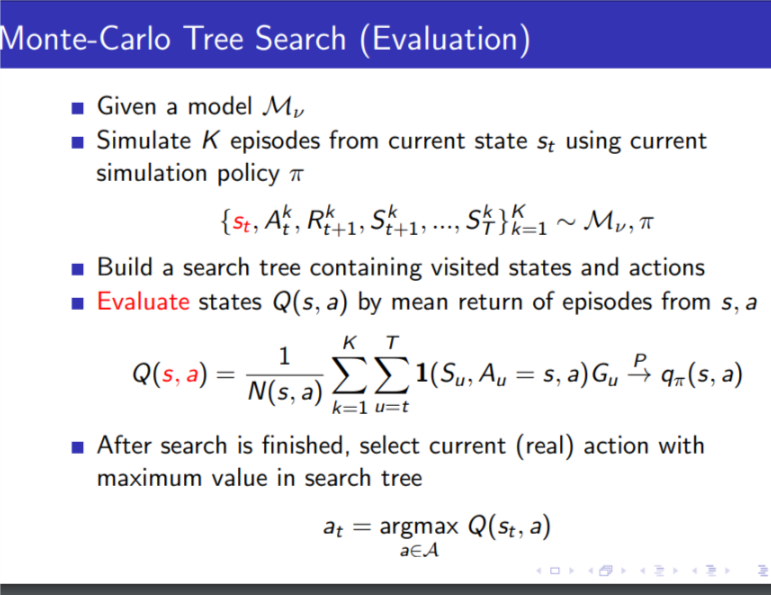
\includegraphics[width = \textwidth]{images/treesearch.png}
        \end{center}
    We then use the information in our tree to make the policy better. 
        \begin{center}
    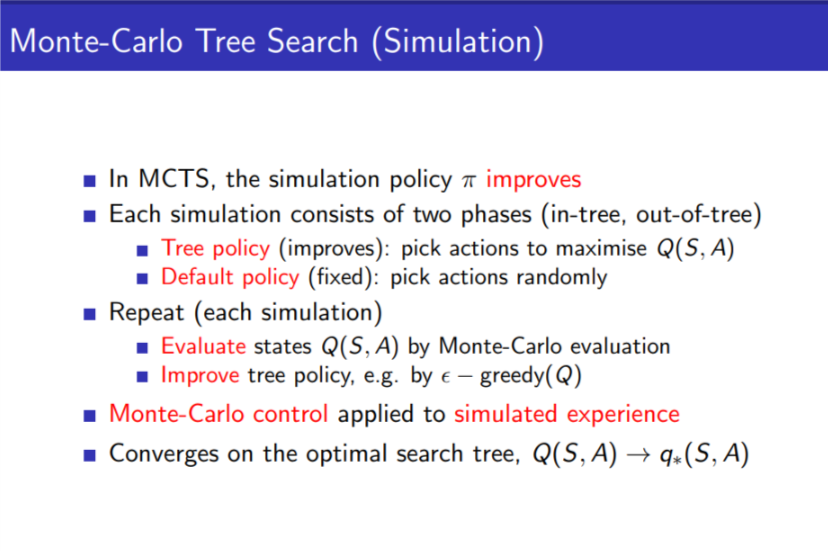
\includegraphics[width = \textwidth]{images/treesim.png}
        \end{center}
        \item Advantages of MC Tree Search. it is highly selective best-first search. It evaluates states dynamically unlike e.g.DP. It uses sampling to break the curse of dimenstionality. it works for black-box models(it only requires samples. Also it is computationally efficient, anytime and parallelizable. 
        \item There is also temporal-difference search. It is also simualation-based search. But we use TD instead of MC. MC tree search applies MC control to sub-MDP from now. TD search applies Sarsa to sub-MDP from now. 
        \item For model-free RL, bootstrapping is helpful. TD learning reduces variance but increases bias. TD learning is usually more efficient than MC. TD(lambda) is much more efficient than MD.For simulation-based search it does the same! 
            \begin{center}
    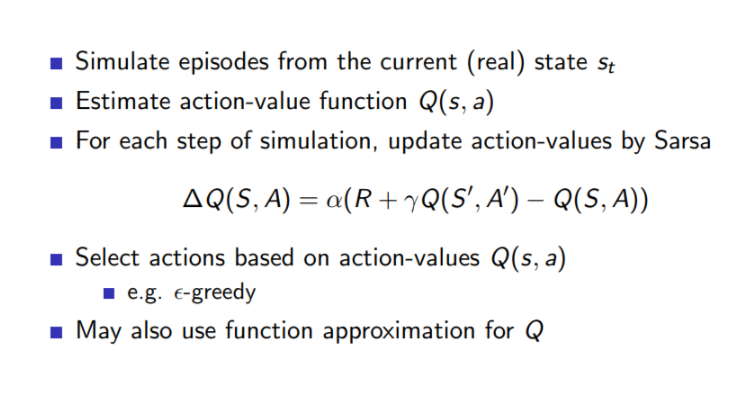
\includegraphics[width = \textwidth]{images/tdsearch.png}
        \end{center}
        \item Remember for both searches, we can also use Functon approximators. 
        \item Dyna-2: the agent stores two sets of feature weights: long-term and short-term memory. The Long term memory is updated from real experience using TD learning. The short term memory is updated from simulated experience using TD search. 
\end{itemize}

section{Exploration and Exploitation}
\begin{itemize}
    \item We will have a look at multi-armed bandits and contextual bandits and lastly MDP's. 
    \tem Online decision making involves a fundamental choice: Exploitation(make the best decision given current information) or exploration(gather more information to get more reward). The best long-term strategy may involve short-term sacrifices to gather enough information to make the best overall decisions. 
    \item We will look at three different exploration techniques. The first is to do random exploration(epsilon-greedy). The next is to use optimism in the face of uncertainty. There you estimate uncertainty on the value and prefer to explore states/actions with highest uncertainty. The last one is information state space usage, that is one considers agent's information as part of its state. We then do look ahead to see how information helps the reward.  So you can say I am in a state where I have tried left three times and right one time. We can then ask how good it is to move into a state where the agent has no or some information. 
    \item There are two types of exploration. There is state-action exploration which tries to systematically explore the state or action space. So we know something about the states and explore based on that. There is also parameter exploration, it parametrizes a policy by a parameter. One could then try different parameters which influence the policy. The advantage of that is we have consistent exploration and the disadvantage is that one doesn't know about the state/action space exploration. So here the exploration part is just that we try different parameters to see how it works.
    \end{itemize}

    \subsection{Multi Armed bandit}
    \begin{itemize}
        \item It's a simplification of the MDP problem. It is a tuple <A,R> where a is a known set of actions. $R^(r)= P[R=r|A=a]$ is an unknown probability distribution over rewards. At each step the agent selects an action and the environment generates a reward. The goal is to maximize the cumulative reward. So the difference is that we throw away the whole state space and the transitions. 
        \item The action-value is the mean reward for action a,$$q(a) = E[R|A = a]$$. The optimal value v* is $$v*= q(a*) = max_{a \epsilon A}q(a) $$
        The regret is the opportunity loss for one step:
        $$l_t = E[v* - q(A_t)]$$
        The total regret is the  total opportunity loss: 
        $$E[\sum_{\tau = 1}^t v* - q(a_{\tau}]$$. The goal is ot maximize the cumulative reward or to minimize the total regret. 
        \item The count $N_t(a)$ is the expected number of selections for action a. The gap is the difference in value between action a and an optimal action a*: $\delta_a = v*-q(a)$
        \item Regret is a function of gaps and the counts $$L_t = E[\sum_{\tau}^t v* - q(A_{\tau}]$$
        $$\sum_{a \epsilon A} E[N_t(a)](v*-q(a))$$
        $$ = \sum_{a \epsilon A} E[N_t(a)]]\delta_a$$
        A good algorithm ensures small counts for large gaps. The problem though is that the gaps are not known. 
        \item If an algorithm forever explores it will hit linear total regret. If an algorithm never explores it will have linear total regret. 
        \item We consider algorithms that estimate $Q_t(a) \sim q(a)$. We estimate the value of each action by Monte-Carlo evaluation: $$Q_t(a) = \frac{1}{N_t(a) }\sum_{t=1}^T 1(A_t = a) R_t$$
        So that means just the mean reward of each action. The greedy algorithm selects the action with the highest value: $$A_t = argmax Q_t(a)$$. Greey can lock onto suboptimal action forever and thus the total regret is linear. 
        \item A first improvement would be to initialize values to the maximum possible, i.e.$Q(a) = r_{max}$. Then act greedily $$a_t = argmax_{a \epsilon A} Q_t(a)$$ This encourages exploration of unknown values, but a few unlucky samples can lock out optimal action forever and thus it also has linear total regret. So the way it actually works is that it is just some kind of bias. We say we have already seen the optimal value a hundred times and then we do the same as before(MC) from there on. 
        \item The epsilon greedy algorithm continues to explore forever. The constant epsilon ensures a minimum regret:$$I_t >= \frac{\epsilon}{|A|}\sum_{a \epsilon A}\delta_a $$. Thus epsilon greedy has a linear total regret. But if we pick a decay schedule for epsil
        on we have logarithmic asymptotic regret. 
        \item So the goal is to find an algorithm with sublinear regret for any multi-armed bandit without knowing the rewards beforehand. 
        \item A hard bandit problem is one with similar distributions but different means. Asymptotic total reward is at least logarithmic in number of steps. 
        \item We will use upper confidence bounds for each action value pair. Such that $q(a) <= Q_t(a) + U_t(a) $ with high probability. This dpends on the number of times N(a) has been selected. A small N(a) implies a large U(a) (estimated value is uncertain). a large N(a) implies a small U(a) (estimated value is accurate.  We then pick the action maximizing the UCB:
        $$ A_t = argmax Q_t(a)  + U_t(a)$$
        \item We apply Hoeffdings inequality to our Upper bound. This gives us: $$U_t(a) = (\frac{-log p}{2N_t(a))}^{1/2} = \frac{2log t}{N_t(a)}^{1/2}$$
        \item This leads to the UCB1 algorithm: 
        $$a_t = argmax Q_t(a) + (\frac{2log t}{N_t(a)})^{1/2}$$ which has logarithmic asymptotic regret. 
        \item Bayesian bandits exploit prior knowledge about rewards. So we consider a distribution over action value functions with parameter w.We then use bayesian methods to compute posterior distributions over w. We can use this  to guide the exploration. Either use it as UCB bound or try to do probability matching which selects an action a according to the probability that a is the optimal action. So for distributions that we do not know a lot about, there is a high chance that an action could be the max for that one. 
        \item What is asymptotically optimal is to sample from your distributions, take the one that is maximal and use that action. That is called Thompson sampling. 
    \end{itemize}
    \subsection{Information Exploration}
    \begin{itemize}
        \item So far we have seen 2 of three methods, randomized exploration and UCB algorithms. 
        \item Exploration is useful because it gains information.Can we quantify the value of information? Can we quantify the long term gain of exploring a trejectory? How much reward a decison-maker would be prepared to pay in order to have that information, prior to making the decision. The long-term reward after getting information - immediate reward. Information gain is higher in uncertain situations. Therefore it make ssense to explroe uncertain situations more.  So the tradeoff of information depends on how much budget we have. if we know the value of information, we can trade-off exploration and exploitation optimally. 
        \item We have viewed bandits as on-step decision-making problems. But it can also be viewed as a sequential decision-making problems. At eacht step there is an information state s which summarizes ll information accumulated so far. Each action A causes a transition to a new information state .
        \item So lets assume a bernoulli bandit such that $R=B(\mu_a)$.We want to find the arm which ahs the highest $\mu_a$. The information state $S= <\alpha, \beta>$ with $\alpha$ counts the pulls of arm a where reward was 0 and $\beta$ counts the pulls of arm a where reward was 1. 
        \item One can do a look ahead ex. for drugs. If it succeeds I would change my success distribution in a certain way and if I fail in another. So we have an infinite MDP over information states. This MDP can be solved by reinforcement learning. 
        \item We begin with a $Beta(\alpha, \beta)$ prior over the reward function R. Each time action a is selected, we update posterior R: $Beta(\alpha +1, Beta)$ if reward is 0 and otherwise if reward is 1. Each information state  corresponds to a model beta. 
    \end{itemize}

    \begin{itemize}
        \item A contextual bandit uses a state. The reward is then dependent on the state and the action. We can estimate the value function with linear function approximators. 
        \item How can we use the things learned today in the full MDP problem. The UCB approach can be generalized so can all the others. For the UCB you would take the Q-value of a state action pair and add some uncertainty part to it. But this ignores that in an MDP we will start to improve our policy. So we shoudl also take into account how much we could improve our policy .
        \item One successful approach to exploration/exploitation in model-based RL is to construct a model of the MDP. For unknown or poorly estimated states, we replace the reward function with the r-max value. That is we are very optimistic in the face of uncertainty and solve optimistic MDP by our favorite planning algorithm(tree search, policy iteration, value iteration etc.). This algo is called Rmax. The information based method can also be applied to MDP's. 
    \end{itemize}
    



\bibliography{reference}
\bibliographystyle{plain}
\end{document}
